\documentclass[12pt]{article}

% =========================
% PREAMBULO (el mismo de la tesis)
% =========================

% Idioma y codificación
\usepackage[spanish,es-tabla]{babel}
\usepackage[utf8]{inputenc}
\usepackage[T1]{fontenc}
\usepackage{mathptmx}
\usepackage{amsmath}
\usepackage{amssymb}
% Tablas bonitas
\usepackage{booktabs}
\usepackage{makecell}
\usepackage{tabularx}
\usepackage[table]{xcolor}
\usepackage{longtable}
\usepackage{array}
\usepackage{amsmath}
\definecolor{headerblue}{RGB}{26,97,133}
\definecolor{lineblue}{RGB}{82,172,220}
\definecolor{rowblue}{RGB}{173,211,230}

\arrayrulecolor{lineblue}
\setlength{\arrayrulewidth}{0.5pt}

\usepackage[ruled,vlined]{algorithm2e}
\newcommand{\headercell}[1]{\textcolor{white}{\textbf{#1}}}
% Control de figuras/tablas y referencias
\usepackage{caption}
\usepackage{subcaption} % subfiguras
\usepackage{tikz}
\usetikzlibrary{arrows.meta, positioning}
% Para que [H] funcione y no se muevan tanto
\usepackage{float}
\usepackage{tikz}
\usepackage{xcolor}
% Links (índice clickeable, referencias clickeables)
\usepackage[colorlinks=true,linkcolor=black,citecolor=black,urlcolor=blue]{hyperref}

% Listas mejoradas
\usepackage{enumitem}
\definecolor{azulESCOM}{RGB}{82,172,220}
% Código (recomendado)
\usepackage{listings}
\usepackage{xcolor}
% Bibliografía IEEE

\usepackage[backend=biber,style=ieee]{biblatex}

% Evita los parentesis vacios "()" en referencias web sin fecha de publicacion
\usepackage{xpatch}
\xpatchbibdriver{online}
  {\printtext[parens]{\usebibmacro{date}}}
  {\iffieldundef{year}{}{\printtext[parens]{\usebibmacro{date}}}}
  {}{}
\addbibresource{references.bib}
\setlength{\parindent}{0pt}%sangria
\setlength{\parskip}{0.4em}

\usepackage{csquotes}

% Gráficos y márgenes
\usepackage{graphicx}
\usepackage[
a4paper,
left=3cm,
right=2cm,
top=2cm,
bottom=2cm
]{geometry}

% Numeracion de tablas y figuras por seccion (Tabla 3.1, Figura 3.2, ...)
\numberwithin{table}{section}
\numberwithin{figure}{section}
\numberwithin{equation}{section}

% Margen de holgura para lineas dificiles de partir (URLs largas en la bibliografia)
\setlength{\emergencystretch}{3em}


% ---- Ajustes propios del manual ----
% Marca visible de "texto por redactar" (se ve en el PDF en gris cursiva)
\newcommand{\pendiente}[1]{\textcolor{gray}{\textit{[Por redactar: #1]}}}
% Estilo para comandos de consola y archivos de configuracion
\lstdefinestyle{consola}{
  basicstyle=\ttfamily\small,
  backgroundcolor=\color{gray!10},
  frame=single, rulecolor=\color{lineblue},
  breaklines=true, columns=fullflexible,
  showstringspaces=false, keepspaces=true,
  upquote=true                 % comillas rectas ' y ` (se pueden copiar a la terminal)
}
\lstset{style=consola}
% Espacio para captura de pantalla.
%   \captura{archivo}{descripcion}
% Si existe images/capturas/<archivo>.png se inserta la imagen; si no, se dibuja un
% recuadro gris con el nombre que debe llevar la captura. Basta con guardar el PNG con ese
% nombre y volver a compilar.
\newcommand{\captura}[2]{%
  \begin{figure}[H]
  \centering
  \IfFileExists{images/capturas/#1.png}%
    {\includegraphics[width=0.92\textwidth,keepaspectratio,height=0.42\textheight]{images/capturas/#1.png}}%
    {\fcolorbox{lineblue}{gray!5}{\parbox[c][4.2cm][c]{0.86\textwidth}{\centering
      \color{gray}\textbf{ESPACIO PARA CAPTURA}\\[6pt]
      \texttt{images/capturas/#1.png}\\[6pt]\small #2}}}
  \caption{#2}\label{fig:#1}
  \end{figure}}
% Nota destacada
\newcommand{\nota}[1]{\par\noindent\fcolorbox{lineblue}{rowblue!25}{\parbox{0.96\textwidth}{\small\textbf{Nota: }#1}}\par\medskip}

\begin{document}
\sloppy

% =========================
% PRELIMINARES
% =========================
%% Portadas (institucional y con resumen) -- las mismas de la tesis

% =========================
% PORTADA
% =========================


\newgeometry{top=2cm, bottom=2cm, right=2cm, left=3cm}

\begin{titlepage}
	\thispagestyle{empty}
	\centering
	
	% --- LÍNEAS Y LOGOS ---
	\begin{tikzpicture}[remember picture, overlay]
		
		% Logo IPN alineado con las líneas azules
		\node[anchor=north] 
		at ([xshift=1.60cm, yshift=-1.25cm]current page.north west) {
			
\includegraphics[width=2.25cm]{images/ipn.png}
		};
		
		% Tres líneas azules entre los logos, como en la plantilla
		% No atraviesan las imágenes
		\foreach \x in {1.45,1.60,1.75} {
			\draw[azulESCOM, line width=1.5pt] 
			([xshift=\x cm, yshift=-3.85cm]current page.north west) -- 
			([xshift=\x cm, yshift=4.20cm]current page.south west);
		}
		
		% Logo ESCOM alineado con las líneas azules
		\node[anchor=south] 
		at ([xshift=1.60cm, yshift=2.0cm]current page.south west) {
			
\includegraphics[width=2.45cm]{images/ESCOM.png}
		};
		
	\end{tikzpicture}
	
	\vspace*{0.85cm}
	
	% --- BLOQUE INSTITUCIONAL ---
	{\fontsize{20}{24}\selectfont \textbf{INSTITUTO POLITÉCNICO NACIONAL}}\\[0.35cm]
	{\fontsize{16}{19.2}\selectfont \textbf{ESCUELA SUPERIOR DE CÓMPUTO}}\\[0.55cm]
	{\fontsize{20}{24}\selectfont \textbf{ESCOM}}\\[1.45cm]
	
	% --- BLOQUE DEL PROYECTO ---
	{\fontsize{14}{16.8}\selectfont \textit{Trabajo Terminal}}\\[0.75cm]
	
	{\fontsize{14}{16.8}\selectfont 2026-B009}\\[0.75cm]
	
	{\fontsize{16}{19.2}\selectfont \bfseries
		``Manual de Instalación de la Plataforma Web para la Denuncia Segura y Prevención de Riesgos Digitales''
	}\\[0.6cm]
	
	\vfill
	
	% --- BLOQUE DE AUTOR ---
	{\fontsize{14}{16.8}\selectfont \textit{Presentan}}\\[0.4cm]
	{\fontsize{14}{16.8}\selectfont \textbf{Edgar Jair Flores Espinosa}}\\[.5cm]
	{\fontsize{14}{16.8}\selectfont \textbf{Jose Bryan Omar Jimenez Velazquez}}\\[.5cm]
	{\fontsize{14}{16.8}\selectfont \textbf{Leilani Shareni Santos Rivera}}\\[.5cm]

	
	% --- BLOQUE DE DIRECTOR ---
	{\fontsize{14}{16.8}\selectfont \textit{Directores}}\\[0.4cm]
	{\fontsize{14}{16.8}\selectfont \textbf{Dr. Jessie Paulina Guzman Flores}}\\[.3cm]
	{\fontsize{14}{16.8}\selectfont \textbf{M. en C. Ulises Velez Saldaña}}\\[.3cm]
	\vfill
	
	% --- PIE DE PÁGINA ---
	{\fontsize{12}{14.4}\selectfont 29 de Diciembre de 2026}
	
\end{titlepage}

\restoregeometry






	
	% =========================
	% PORTADA ADICIONAL CON RESUMEN
	% =========================
	\begin{titlepage}
		\thispagestyle{empty}
		
		\begin{center}
			
			% Encabezado bien alineado
			\noindent
			\begin{minipage}[c]{0.18\textwidth}
				\centering
				
\includegraphics[width=2.4cm]{images/ipn.png}
			\end{minipage}
			\begin{minipage}[c]{0.62\textwidth}
				\centering
				{\fontsize{20}{22}\selectfont \textbf{INSTITUTO POLITÉCNICO NACIONAL}\par}
				{\fontsize{16}{18}\selectfont \textbf{ESCUELA SUPERIOR DE CÓMPUTO}\par}
				{\fontsize{16}{18}\selectfont \textbf{SUBDIRECCIÓN ACADÉMICA}\par}
			\end{minipage}
			\begin{minipage}[c]{0.18\textwidth}
				\centering
				
\includegraphics[width=3.0cm]{images/ESCOM.png}
			\end{minipage}
			
			\vspace{0.9cm}
			
			\noindent
			\begin{minipage}{0.45\textwidth}
				\raggedright
				{\fontsize{14}{16}\selectfont No. de TT: 2026-B009}
			\end{minipage}
			\begin{minipage}{0.50\textwidth}
				\raggedleft
				{\fontsize{14}{16}\selectfont Fecha de presentación de TT-II: 05 de junio de 2026}
			\end{minipage}
			
			\vspace{0.55cm}
			
			{\fontsize{14}{16}\selectfont Documento Técnico\par}
			
			\vspace{0.65cm}
			
			\begin{minipage}{0.88\textwidth}
				\centering
				{\fontsize{16}{18}\selectfont \textbf{``Manual de Instalación de la iPlataforma Web para la Denuncia Segura y Prevención de Riesgos Digitales''}\par}
			\end{minipage}
			
			\vspace{1.25cm}
			
			{\fontsize{14}{16}\selectfont \textit{Presentan:}\par}
			\vspace{0.15cm}
			{\fontsize{14}{16}\selectfont \textbf{Edgar Jair Flores Espinosa, Jose Bryan Omar Jimenez Velazquez, Leilani Shareni Santos Rivera}\par}
			
			\vspace{1.35cm}
			
			{\fontsize{14}{16}\selectfont \textit{Directores:}\par}
			
			\vspace{0.45cm}
			
			{\fontsize{14}{16}\selectfont \textbf{Dr. Jessie Paulina Guzman Flores}\par}
			{\fontsize{14}{16}\selectfont \textbf{M. en C. Ulises Velez Saldaña}\par}
						
			\vspace{1.1cm}
			
			{\fontsize{14}{16}\selectfont \textbf{MANUAL DE INSTALACION}\par}
			
		\end{center}
		
		\vspace{0.25cm}
		
		\vfill
		
		{\fontsize{12}{14}\selectfont
			\rule{6cm}{0.4pt}\\[-0.05cm]
			\textsuperscript{1}\texttt{josebryanomar2004@gmail.com}
		}
		
	\end{titlepage}


%% Indice general, de figuras y de tablas
	% Numeración romana para preliminares
	
	\pagenumbering{roman}
	
	\tableofcontents
	\newpage
	
	\listoffigures
	\newpage
	
	\listoftables
	\newpage
	
	% Numeración arábiga para el contenido
	\pagenumbering{arabic}
	
	


% =========================
% CONTENIDO DEL MANUAL
% (un capitulo por carpeta en capitulos/; la version anterior queda en sections/manual)
% =========================
% Capítulo 1. Introducción y Arquitectura Distribuida
\section{Introducción y Arquitectura Distribuida}\label{cap:01_introduccion_arquitectura}
Este capítulo presenta la plataforma que se instala con este manual, la forma en que sus componentes se reparten entre tres servidores virtuales (VPS) y la manera en que se comunican entre sí. Sirve como mapa de referencia para el resto del documento: cada capítulo posterior instala una de las piezas que aquí se describen.

% Resumen de la solución
\subsection{Resumen de la solución}\label{sec:1_1_resumen_solucion}

\subsubsection{Descripción general de la plataforma (microservicios Spring Boot, frontends Angular y modelo de IA)}
La Plataforma de Quejas de la Defensoría de los Derechos Politécnicos (DDP) es un sistema web que permite a la comunidad del Instituto Politécnico Nacional presentar quejas y darles seguimiento, y al personal de la Defensoría recibirlas, revisarlas, turnarlas y atenderlas. Está construida con una arquitectura de microservicios y se compone de tres tipos de piezas:

\begin{itemize}
  \item \textbf{Microservicios (backend).} Diez servicios independientes desarrollados en Java 21 con Spring Boot. Cada uno resuelve una parte del negocio, expone una API REST y se ejecuta en su propio contenedor de Podman.
  \item \textbf{Frontends (interfaz web).} Cinco aplicaciones Angular, una por cada tipo de usuario. Se compilan a archivos estáticos (HTML, CSS y JavaScript) y cada una se sirve desde su propio contenedor de nginx.
  \item \textbf{Modelo de inteligencia artificial.} El servicio \texttt{antecedentes-service}, también en Java, busca quejas parecidas en el histórico mediante TF-IDF y similitud coseno, y genera un resumen extractivo de cada queja con TextRank. No requiere GPU ni servicios externos.
\end{itemize}

Todos los servicios guardan su información en una sola base de datos PostgreSQL 16 (\texttt{defensoria\_db}).

\begin{table}[H]
\centering
\caption{Microservicios de la plataforma}
\small
\begin{tabular}{p{4.3cm}p{10.2cm}}
\toprule
\textbf{Servicio} & \textbf{Función} \\
\midrule
\texttt{auth-service} & Inicio de sesión, emisión de tokens JWT, activación de cuentas y recuperación de contraseña \\
\texttt{quejas-service} & Registro y consulta de quejas, folios, credenciales y evidencias \\
\texttt{notificaciones-service} & Avisos dentro de la plataforma y envío de correos \\
\texttt{catalogo-service} & Catálogo de dependencias (unidades académicas) del IPN \\
\texttt{admin-service} & Panel de la Defensora: indicadores, personal, configuración y respaldos \\
\texttt{revision-service} & Validación por la recepcionista y turnado de quejas \\
\texttt{chatbot-service} & Preguntas frecuentes del asistente del portal \\
\texttt{denunciado-service} & Registro de la respuesta y evidencias de la persona denunciada \\
\texttt{primer-contacto-service} & Módulo de Primer Contacto (atención inicial y citas) \\
\texttt{subdefensoria-service} & Módulo de la Subdefensoría (atención de quejas turnadas) \\
\texttt{antecedentes-service} & Modelo de IA: búsqueda de antecedentes y resumen de quejas \\
\bottomrule
\end{tabular}
\end{table}

\begin{table}[H]
\centering
\caption{Frontends de la plataforma}
\small
\begin{tabular}{p{4.3cm}p{3.4cm}p{6.5cm}}
\toprule
\textbf{Frontend} & \textbf{Ruta pública} & \textbf{Usuarios} \\
\midrule
Portal (\texttt{defensoria-web}) & \texttt{/} & Quejosos y personas denunciadas \\
Revisión (\texttt{revision-web}) & \texttt{/revision/} & Login unificado del personal y recepcionistas \\
Administración (\texttt{admin-web}) & \texttt{/admin/} & Defensora y administración del sistema \\
Primer Contacto (\texttt{primer-contacto-web}) & \texttt{/primer-contacto/} & Analistas de Primer Contacto \\
Subdefensoría (\texttt{subdefensoria-web}) & \texttt{/subdefensoria/} & Abogados de la Subdefensoría \\
\bottomrule
\end{tabular}
\end{table}

\subsubsection{Objetivo del despliegue en 3 VPS}
El objetivo del despliegue es dejar la plataforma completa en producción y accesible en \url{https://defensoria-escom.ddns.net}, separando sus componentes en tres servidores virtuales, uno por capa:

\begin{itemize}
  \item \textbf{Seguridad.} Solo el servidor frontend queda expuesto a Internet. El backend acepta conexiones únicamente del frontend, y la base de datos únicamente del backend, de modo que los datos de las quejas nunca quedan directamente al alcance de un atacante externo.
  \item \textbf{Aislamiento de recursos.} La base de datos, los microservicios y los portales no compiten por la misma memoria y CPU; si un servicio consume más de lo previsto, no afecta a las otras capas.
  \item \textbf{Mantenimiento independiente.} Cada capa se puede actualizar, reiniciar o respaldar sin detener a las demás.
  \item \textbf{Reproducibilidad.} Todos los componentes se ejecutan en contenedores Podman creados con scripts, por lo que la instalación se puede repetir de la misma forma en servidores nuevos.
\end{itemize}

\begin{table}[H]
\centering
\caption{Servidores del despliegue}
\small
\begin{tabular}{llll}
\toprule
\textbf{Capa} & \textbf{Hostname} & \textbf{IP pública} & \textbf{Contenido} \\
\midrule
Frontend & vmi3633026 & 169.58.62.111 & router-nginx y 5 frontends \\
Backend & vmi3633021 & 156.67.26.73 & 10 microservicios y modelo de IA \\
Base de datos & vmi3633025 & 169.58.62.99 & PostgreSQL 16 (\texttt{defensoria-db}) \\
\bottomrule
\end{tabular}
\end{table}

% Diagrama de arquitectura en 3 capas
\subsection{Diagrama de arquitectura en 3 capas}\label{sec:1_2_diagrama_arquitectura}

\subsubsection{Relación entre VPS Frontend (router-nginx y frontends), VPS Backend (microservicios y modelo de IA) y VPS Base de Datos (PostgreSQL)}
La plataforma sigue una arquitectura de tres capas en la que cada capa vive en su propia VPS y solo se comunica con la capa contigua (Figura \ref{fig:arquitectura-3-capas}).

\begin{figure}[H]
\centering
\resizebox{\textwidth}{!}{%
\begin{tikzpicture}[
  vps/.style={draw=headerblue, thick, rounded corners, fill=rowblue!15, minimum width=4.6cm, minimum height=6.9cm, anchor=north},
  comp/.style={draw=headerblue, fill=white, rounded corners, align=center, minimum width=3.9cm, minimum height=0.62cm, font=\scriptsize},
  user/.style={draw=headerblue, fill=rowblue!40, rounded corners, align=center, minimum width=2.4cm, minimum height=1.2cm, font=\small},
  flecha/.style={-latex, thick, headerblue}]
  % Usuario
  \node[user] (u) at (-4.2,-4.1) {Usuario\\(navegador)};
  % VPS Frontend
  \node[vps] (f) at (0.6,0) {};
  \node[font=\small\bfseries, align=center] at (0.6,-0.45) {VPS Frontend\\[-2pt]\scriptsize 169.58.62.111};
  \node[comp, fill=rowblue!40] (rn) at (0.6,-1.6) {\textbf{router-nginx} (80/443)\\HTTPS, proxy inverso};
  \node[comp] at (0.6,-2.9) {defensoria-web (8090)};
  \node[comp] at (0.6,-3.65) {admin-web (8091)};
  \node[comp] at (0.6,-4.4) {revision-web (8092)};
  \node[comp] at (0.6,-5.15) {primer-contacto-web (8094)};
  \node[comp] at (0.6,-5.9) {subdefensoria-web (8095)};
  % VPS Backend
  \node[vps] (b) at (6.6,0) {};
  \node[font=\small\bfseries, align=center] at (6.6,-0.45) {VPS Backend\\[-2pt]\scriptsize 156.67.26.73};
  \node[comp] at (6.6,-1.4) {auth (8083) \quad quejas (8084)};
  \node[comp] at (6.6,-2.15) {notificaciones (8085) \quad catálogo (8086)};
  \node[comp] at (6.6,-2.9) {admin (8087) \quad revisión (8088)};
  \node[comp] at (6.6,-3.65) {chatbot (8089) \quad denunciado (8094)};
  \node[comp] at (6.6,-4.4) {primer contacto (8082)};
  \node[comp] at (6.6,-5.15) {subdefensoría (8091)};
  \node[comp, fill=rowblue!40] (ia) at (6.6,-6.1) {\textbf{antecedentes-service} (8093)\\modelo de IA};
  % VPS BD
  \node[vps, minimum height=4.2cm] (d) at (12.6,-2) {};
  \node[font=\small\bfseries, align=center] at (12.6,-2.45) {VPS Base de Datos\\[-2pt]\scriptsize 169.58.62.99};
  \node[comp, fill=rowblue!40, minimum height=1.2cm] (db) at (12.6,-4.1) {\textbf{defensoria-db}\\PostgreSQL 16 (5432)\\\texttt{defensoria\_db}};
  % Flechas
  \draw[flecha] (u) -- node[below, font=\scriptsize, yshift=-12pt]{HTTPS 443} (-1.7,-4.1);
  \draw[flecha] (2.9,-4.1) -- node[above, font=\scriptsize, align=center]{/api/*\\8082--8094} (4.3,-4.1);
  \draw[flecha] (8.9,-4.1) -- node[above, font=\scriptsize, align=center]{JDBC\\5432} (10.3,-4.1);
\end{tikzpicture}}
\caption{Arquitectura de la plataforma en 3 capas}\label{fig:arquitectura-3-capas}
\end{figure}

\begin{itemize}
  \item \textbf{VPS Frontend.} Es la única capa visible desde Internet. El contenedor \texttt{router-nginx} recibe todo el tráfico en los puertos 80 y 443, termina la conexión cifrada (HTTPS) con el certificado de Let's Encrypt y decide a dónde enviar cada petición: las páginas se las pide a uno de los cinco contenedores de frontend que corren en el mismo servidor, y las llamadas que empiezan con \texttt{/api/} las reenvía al backend.
  \item \textbf{VPS Backend.} Ejecuta los diez microservicios y el modelo de IA, cada uno en su contenedor. Recibe peticiones solo del frontend. Los microservicios también se llaman entre sí; por ejemplo, \texttt{quejas-service} avisa a \texttt{notificaciones-service} cuando se registra una queja, y \texttt{primer-contacto-service} consulta a \texttt{antecedentes-service} para buscar antecedentes de una queja.
  \item \textbf{VPS Base de Datos.} Ejecuta PostgreSQL 16 en el contenedor \texttt{defensoria-db}, con la base \texttt{defensoria\_db}. Solo acepta conexiones del backend. Las tablas las crea cada microservicio al arrancar (Hibernate).
\end{itemize}

\subsubsection{Flujo de una petición del usuario}
Como ejemplo, se sigue el recorrido completo cuando una persona registra una queja desde el portal:

\begin{enumerate}
  \item El usuario abre \url{https://defensoria-escom.ddns.net}. El dominio de No-IP resuelve a la IP del VPS Frontend (169.58.62.111).
  \item \texttt{router-nginx} recibe la petición en el puerto 443, establece la conexión HTTPS y, como la ruta es \texttt{/}, la envía a \texttt{defensoria-web} (\texttt{127.0.0.1:8090}), que devuelve la aplicación Angular del portal.
  \item El usuario llena el formulario y lo envía. El navegador hace una petición \texttt{POST} a \texttt{/api/quejoso/...} con los datos de la queja, su credencial y sus evidencias.
  \item \texttt{router-nginx} identifica la ruta \texttt{/api/quejoso/} y reenvía la petición al VPS Backend, a \texttt{156.67.26.73:8084} (\texttt{quejas-service}). El firewall del backend la acepta porque proviene de la IP del frontend.
  \item \texttt{quejas-service} valida la información, genera el folio y guarda la queja y sus archivos en \texttt{defensoria\_db} a través de JDBC hacia \texttt{169.58.62.99:5432}. El firewall de la base la acepta porque proviene de la IP del backend.
  \item \texttt{quejas-service} llama a \texttt{notificaciones-service} (puerto 8085) para registrar el aviso correspondiente.
  \item La respuesta con el folio regresa por el mismo camino: backend $\rightarrow$ \texttt{router-nginx} $\rightarrow$ navegador, y el portal muestra el folio al usuario.
\end{enumerate}

Las peticiones del personal siguen el mismo patrón; la diferencia es que incluyen el token JWT emitido por \texttt{auth-service}, que cada microservicio valida con el secreto compartido antes de responder.

% Matriz de conectividad y puertos
\subsection{Matriz de conectividad y puertos}\label{sec:1_3_matriz_conectividad}

\subsubsection{Direccionamiento IP público por VPS (169.58.62.111, 156.67.26.73, 169.58.62.99)}
Cada VPS cuenta con una sola dirección IP pública. Las tres se comunican entre sí por esas direcciones; no existe una red privada entre ellas, por lo que el aislamiento de cada capa se logra con reglas de firewall que solo aceptan tráfico de la IP de la capa anterior (capítulo \ref{cap:03_seguridad_red_firewall}).

\begin{table}[H]
\centering
\caption{Direccionamiento y accesos permitidos por VPS}
\small
\begin{tabular}{p{2.3cm}p{2.5cm}p{4.6cm}p{4.6cm}}
\toprule
\textbf{VPS} & \textbf{IP pública} & \textbf{Acepta conexiones de} & \textbf{Se conecta a} \\
\midrule
Frontend & 169.58.62.111 & Internet (80 y 443) & Backend (8082--8094) \\
Backend & 156.67.26.73 & Frontend (8082--8094) y el propio backend & Base de datos (5432); servidor SMTP para correos \\
Base de datos & 169.58.62.99 & Backend (5432) & -- \\
\bottomrule
\end{tabular}
\end{table}

El acceso de administración por SSH (puerto 22) está disponible en las tres VPS. El dominio público \texttt{defensoria-escom.ddns.net} apunta únicamente al VPS Frontend.

\subsubsection{Mapeo de puertos del host y de los contenedores (80/443 router-nginx; 8090--8095 frontends; 8082--8094 microservicios; 5432 defensoria-db)}
Cada contenedor escucha en un puerto interno y Podman lo publica en un puerto del servidor (host). Todos los microservicios escuchan internamente en el 8080, y es el puerto del host el que los distingue. \texttt{router-nginx} no publica puertos: usa la red del host (\texttt{-{}-network host}) para escuchar directamente en el 80 y el 443.

{\small
\begin{longtable}{p{2.1cm}p{4.4cm}p{2.3cm}p{2.3cm}p{2.9cm}}
\caption{Mapeo de puertos del host y del contenedor}\\
\toprule
\textbf{VPS} & \textbf{Contenedor} & \textbf{Puerto host} & \textbf{Puerto contenedor} & \textbf{Imagen base} \\
\midrule
\endfirsthead
\toprule
\textbf{VPS} & \textbf{Contenedor} & \textbf{Puerto host} & \textbf{Puerto contenedor} & \textbf{Imagen base} \\
\midrule
\endhead
Frontend & router-nginx & 80, 443 & red del host & nginx:alpine \\
Frontend & defensoria-web & 8090 & 8090 & nginx:alpine \\
Frontend & admin-web & 8091 & 80 & nginx:alpine \\
Frontend & revision-web & 8092 & 80 & nginx:alpine \\
Frontend & primer-contacto-web & 8094 & 80 & nginx:alpine \\
Frontend & subdefensoria-web & 8095 & 80 & nginx:alpine \\
\midrule
Backend & primer-contacto-service & 8082 & 8080 & eclipse-temurin:21 \\
Backend & auth-service & 8083 & 8080 & eclipse-temurin:21 \\
Backend & quejas-service & 8084 & 8080 & eclipse-temurin:21 \\
Backend & notificaciones-service & 8085 & 8080 & eclipse-temurin:21 \\
Backend & catalogo-service & 8086 & 8080 & eclipse-temurin:21 \\
Backend & admin-service & 8087 & 8080 & eclipse-temurin:21 \\
Backend & revision-service & 8088 & 8080 & eclipse-temurin:21 \\
Backend & chatbot-service & 8089 & 8080 & eclipse-temurin:21 \\
Backend & subdefensoria-service & 8091 & 8080 & eclipse-temurin:21 \\
Backend & antecedentes-service & 8093 & 8080 & eclipse-temurin:21 \\
Backend & denunciado-service & 8094 & 8080 & eclipse-temurin:21 \\
\midrule
Base de datos & defensoria-db & 5432 & 5432 & postgres:16-alpine \\
\bottomrule
\end{longtable}}

\nota{Los puertos 8091 y 8094 aparecen tanto en el frontend como en el backend. No hay conflicto porque están en servidores distintos: en el frontend corresponden a \texttt{admin-web} y \texttt{primer-contacto-web}, y en el backend a \texttt{subdefensoria-service} y \texttt{denunciado-service}.}

\subsubsection{Rutas públicas de nginx hacia cada servicio}
El usuario nunca usa los puertos directamente: todo entra por \url{https://defensoria-escom.ddns.net} y \texttt{router-nginx} decide el destino según la ruta de la URL. Las rutas de los frontends se dirigen a contenedores del mismo VPS (\texttt{127.0.0.1}) y las de la API al VPS Backend.

\begin{table}[H]
\centering
\caption{Rutas públicas de router-nginx}
\small
\begin{tabular}{p{4.6cm}p{4.2cm}p{5.2cm}}
\toprule
\textbf{Ruta pública} & \textbf{Destino} & \textbf{Servicio} \\
\midrule
\multicolumn{3}{l}{\textit{Frontends}} \\
\texttt{/} & \texttt{127.0.0.1:8090} & defensoria-web \\
\texttt{/admin/} & \texttt{127.0.0.1:8091} & admin-web \\
\texttt{/revision/} & \texttt{127.0.0.1:8092} & revision-web \\
\texttt{/primer-contacto/} & \texttt{127.0.0.1:8094} & primer-contacto-web \\
\texttt{/subdefensoria/} & \texttt{127.0.0.1:8095} & subdefensoria-web \\
\midrule
\multicolumn{3}{l}{\textit{API}} \\
\texttt{/api/auth/} & \texttt{156.67.26.73:8083} & auth-service \\
\texttt{/api/quejoso/} & \texttt{156.67.26.73:8084} & quejas-service \\
\texttt{/api/notificaciones/} & \texttt{156.67.26.73:8085} & notificaciones-service \\
\texttt{/api/catalogos/} & \texttt{156.67.26.73:8086} & catalogo-service \\
\texttt{/api/admin/} & \texttt{156.67.26.73:8087} & admin-service \\
\texttt{/api/revision/} & \texttt{156.67.26.73:8088} & revision-service \\
\texttt{/api/chatbot/} & \texttt{156.67.26.73:8089} & chatbot-service \\
\texttt{/api/primer-contacto/} & \texttt{156.67.26.73:8082} & primer-contacto-service \\
\texttt{/api/subdefensoria/} & \texttt{156.67.26.73:8091} & subdefensoria-service \\
\texttt{/api/denunciado/} & \texttt{156.67.26.73:8094} & denunciado-service \\
\bottomrule
\end{tabular}
\end{table}

Además, \texttt{router-nginx} responde \texttt{403} (prohibido) a las siguientes rutas, que son de uso interno entre microservicios:
\begin{itemize}
  \item \nolinkurl{/api/notificaciones/enviar} y \nolinkurl{/api/notificaciones/registrar}
  \item \nolinkurl{/api/primer-contacto/ingesta/}
  \item \nolinkurl{/api/subdefensoria/ingesta/}
  \item \nolinkurl{/api/subdefensoria/acuerdos-conclusion/interno/}
\end{itemize}

El modelo de IA (\texttt{antecedentes-service}, puerto 8093) no tiene ruta pública: solo lo consumen otros microservicios dentro del backend. Las rutas bloqueadas existen porque esos endpoints están pensados para llamadas entre servicios; si quedaran expuestos, cualquier persona podría, por ejemplo, enviar correos desde la cuenta de la Defensoría.


% Capítulo 2. Preparación de Nodos y Entorno de Ejecución (Común a las 3 VPS)
\section{Preparación de Nodos y Entorno de Ejecución (Común a las 3 VPS)}\label{cap:02_preparacion_nodos}
Antes de instalar cualquier componente de la plataforma, las tres VPS se dejan en un mismo estado base: acceso de administración configurado, sistema actualizado, misma zona horaria, Podman instalado y la estructura de carpetas creada con sus permisos. Los pasos de este capítulo se ejecutan en el VPS Frontend (169.58.62.111), el VPS Backend (156.67.26.73) y el VPS Base de Datos (169.58.62.99); cuando un paso aplica solo a uno de ellos, se indica.

% Actualización base y acceso a los servidores
\subsection{Actualización base y acceso a los servidores}\label{sec:2_1_actualizacion_acceso}
Las tres VPS son servidores con Ubuntu 24.04.5 LTS contratados con el proveedor Contabo. La administración se realiza de forma remota por SSH con el cliente Termius, usando la cuenta \texttt{root}. Esta sección explica primero cómo se configura ese acceso y después la actualización del sistema y la zona horaria, que es lo primero que se ejecuta al entrar a cada servidor.

\subsubsection{Acceso por SSH como root con Termius}
\paragraph{Cliente utilizado.} Termius es un cliente SSH gráfico para Windows, macOS y Linux que guarda la lista de servidores con sus credenciales, abre cada conexión en una pestaña o en paneles dentro de un mismo espacio de trabajo (\emph{Workspace}) e incluye un explorador SFTP para transferir archivos. Se utiliza en lugar de la terminal del sistema para tener en un solo lugar las tres VPS de la plataforma y trabajar con ellas al mismo tiempo.

\paragraph{Registro de los servidores.} En Termius se crea un \emph{host} por cada VPS desde \textbf{Hosts $\rightarrow$ New host}, con los siguientes datos:

\begin{table}[H]
\centering
\caption{Hosts registrados en Termius}
\small
\begin{tabular}{llccc}
\toprule
\textbf{Label (nombre)} & \textbf{Address} & \textbf{Puerto SSH} & \textbf{Usuario} & \textbf{Autenticación} \\
\midrule
FRONTEND DEFENSORIA & 169.58.62.111 & 22 & root & Contraseña \\
BACKEND DEFENSORIA & 156.67.26.73 & 22 & root & Contraseña \\
BASE DEFENSORIA & 169.58.62.99 & 22 & root & Contraseña \\
\bottomrule
\end{tabular}
\end{table}

\begin{enumerate}
  \item En \textbf{Address} se escribe la IP pública de la VPS.
  \item En \textbf{General} se asigna el nombre con el que aparecerá en la lista (\emph{Label}).
  \item En \textbf{SSH on port} se deja el puerto \texttt{22}.
  \item En \textbf{Credentials} se captura el usuario \texttt{root} y su contraseña. Termius la guarda cifrada en su bóveda (\emph{vault}) personal, por lo que no es necesario escribirla en cada conexión.
  \item Se guarda el host y se repite para las otras dos VPS.
\end{enumerate}

\begin{figure}[H]
\centering
\begin{subfigure}[t]{0.31\textwidth}\centering
  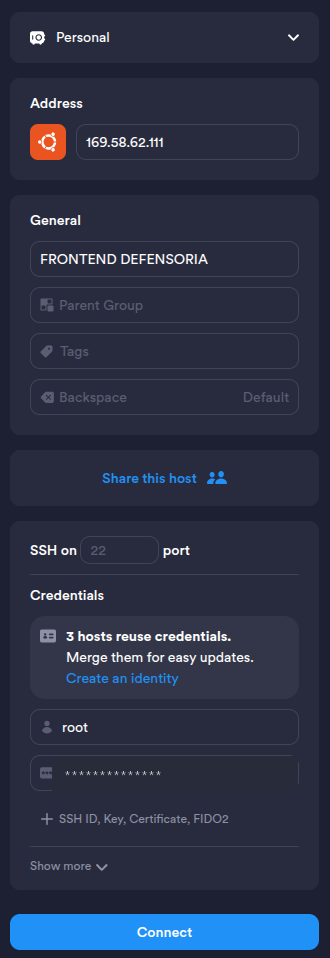
\includegraphics[width=\textwidth]{images/capturas/prep-02-termius-frontend.png}
  \caption{VPS Frontend}
\end{subfigure}\hfill
\begin{subfigure}[t]{0.31\textwidth}\centering
  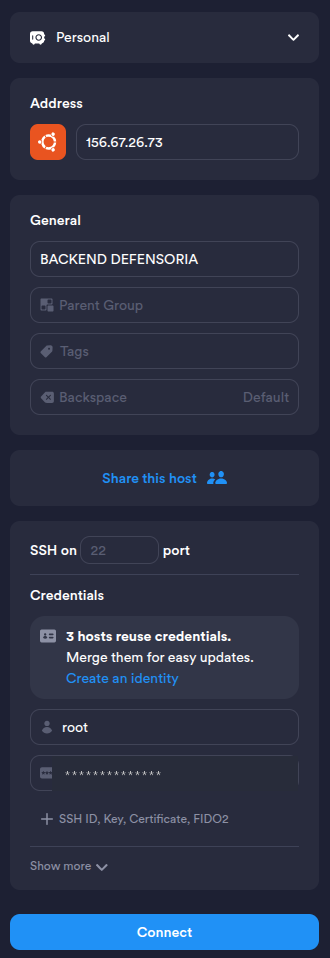
\includegraphics[width=\textwidth]{images/capturas/prep-03-termius-backend.png}
  \caption{VPS Backend}
\end{subfigure}\hfill
\begin{subfigure}[t]{0.31\textwidth}\centering
  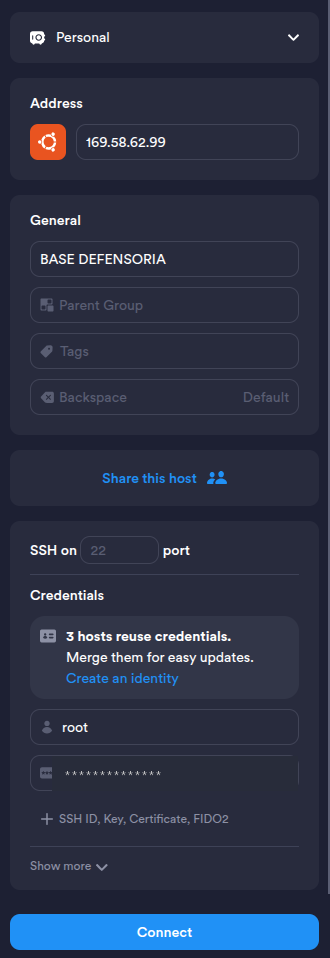
\includegraphics[width=\textwidth]{images/capturas/prep-04-termius-bd.png}
  \caption{VPS Base de Datos}
\end{subfigure}
\caption{Configuración de los tres hosts en Termius (contraseña oculta)}\label{fig:termius-hosts}
\end{figure}

\paragraph{Conexión a las tres VPS.} Al seleccionar un host y pulsar \textbf{Connect}, Termius abre la sesión SSH. En la primera conexión muestra la huella digital (\emph{fingerprint}) de la llave del servidor y pide confirmarla; al aceptarla la registra en \textbf{Known Hosts}. Si en una conexión posterior la huella cambia sin que el servidor se haya reinstalado, se debe rechazar la conexión, porque puede tratarse de un servidor suplantado.

Para la instalación conviene abrir las tres sesiones en un mismo \emph{Workspace}, de modo que las tres VPS quedan visibles a la vez (Figura \ref{fig:prep-05-termius-conexion}). El \emph{prompt} de cada panel muestra el nombre de host del servidor (\texttt{root@vmi3633026}, \texttt{root@vmi3633021}, \texttt{root@vmi3633025}), lo que permite confirmar en qué VPS se está escribiendo antes de ejecutar un comando. La opción \textbf{Broadcast} de Termius envía lo que se escribe a todos los paneles a la vez y sirve para los pasos idénticos en las tres VPS (actualización, zona horaria, instalación de Podman).

\captura{prep-05-termius-conexion}{Sesión SSH como root en las tres VPS dentro de un Workspace de Termius}

\nota{El acceso se hace con usuario \texttt{root} y contraseña, sin llaves SSH. Se recomienda que la contraseña sea larga (16 caracteres o más) y distinta en cada VPS: Termius advierte en la Figura \ref{fig:termius-hosts} que los tres hosts reutilizan las mismas credenciales, de modo que si una se filtra quedan expuestos los tres servidores. Las contraseñas no se escriben en este manual y, al tomar capturas de Termius, el campo de contraseña debe quedar oculto.}

\subsubsection{Actualización del sistema y zona horaria (America/Mexico\_City)}
\paragraph{Actualización de paquetes.} Al conectarse, Ubuntu indica en el mensaje de bienvenida cuántas actualizaciones están pendientes (entre 12 y 14 en la Figura \ref{fig:prep-05-termius-conexion}). En cada VPS se actualiza la lista de paquetes y se instalan:
\begin{lstlisting}
# apt update
# apt upgrade -y
\end{lstlisting}
Si la actualización incluyó un kernel nuevo, Ubuntu crea el archivo \texttt{/var/run/reboot-required}; en ese caso se reinicia la VPS y se vuelve a conectar desde Termius:
\begin{lstlisting}
# [ -f /var/run/reboot-required ] && reboot
\end{lstlisting}

\nota{El mensaje de bienvenida también ofrece actualizar a Ubuntu 26.04 LTS (\texttt{do-release-upgrade}). \textbf{No} se aplica: la plataforma se instaló y probó sobre Ubuntu 24.04 LTS, que sigue recibiendo actualizaciones de seguridad; un cambio de versión mayor se planea por separado.}

\captura{prep-06-apt-upgrade-frontend}{Actualización del sistema en el VPS Frontend}
\captura{prep-07-apt-upgrade-backend}{Actualización del sistema en el VPS Backend}
\captura{prep-08-apt-upgrade-bd}{Actualización del sistema en el VPS Base de Datos}

\paragraph{Zona horaria.} Las VPS vienen con la zona horaria del centro de datos de Contabo en Europa; por eso el mensaje de bienvenida de la Figura \ref{fig:prep-05-termius-conexion} muestra la hora en \texttt{CET}. Se cambian a la hora del centro de México para que las fechas de los registros del sistema, de los logs de los contenedores y de los respaldos coincidan con la hora local de la Defensoría (por ejemplo, el respaldo diario programado a las 4:00 se ejecuta a las 4:00 hora de México y no a media noche):
\begin{lstlisting}
# timedatectl set-timezone America/Mexico_City
# timedatectl
\end{lstlisting}
La salida de \texttt{timedatectl} debe mostrar \texttt{Time zone: America/Mexico\_City (CST, -0600)} y \texttt{System clock synchronized: yes}; esto último indica que el reloj se sincroniza automáticamente por NTP.

\captura{prep-09-zona-horaria-frontend}{Zona horaria America/Mexico\_City en el VPS Frontend}
\captura{prep-10-zona-horaria-backend}{Zona horaria America/Mexico\_City en el VPS Backend}
\captura{prep-11-zona-horaria-bd}{Zona horaria America/Mexico\_City en el VPS Base de Datos}

\nota{La base de datos también trabaja en esta zona horaria: el contenedor \texttt{defensoria-db} se crea con \texttt{TZ=America/Mexico\_City} y el script de inicialización fija la misma zona en \texttt{defensoria\_db} (capítulo \ref{cap:05_despliegue_base_datos}).}

% Instalación y aprovisionamiento de Podman
\subsection{Instalación y aprovisionamiento de Podman}\label{sec:2_2_instalacion_podman}
Todos los componentes de la plataforma (base de datos, microservicios, modelo de IA, frontends y nginx) se ejecutan en contenedores. Como motor de contenedores se usa Podman, que es compatible con las imágenes y los Dockerfile de Docker pero no necesita un proceso servidor (\emph{daemon}) permanente: cada contenedor es un proceso más del sistema, lo que reduce el consumo de memoria en VPS pequeñas.

\subsubsection{Instalación de Podman y utilerías (podman, curl, iptables, python3, certbot)}
En las \textbf{tres} VPS se instalan Podman y las utilerías que usan los scripts de la plataforma:
\begin{lstlisting}
# apt install -y podman curl iptables
# podman --version
\end{lstlisting}
\begin{itemize}
  \item \texttt{podman}: motor de contenedores. Ubuntu 24.04 instala la versión 4.9.
  \item \texttt{curl}: pruebas de los servicios desde la terminal (\texttt{curl http://127.0.0.1:<puerto>}).
  \item \texttt{iptables}: reglas de firewall que aplican los scripts de la plataforma (capítulo \ref{cap:03_seguridad_red_firewall}).
\end{itemize}

Además, según el servidor:
\begin{lstlisting}
# apt install -y python3            # solo VPS Backend
# apt install -y certbot            # solo VPS Frontend
\end{lstlisting}
\begin{itemize}
  \item \texttt{python3} (Backend): lo usa el generador de la carga masiva de quejas (\texttt{generar-csv.py}).
  \item \texttt{certbot} (Frontend): emisión y renovación del certificado HTTPS (sección \ref{sec:7_3_certificados_certbot}).
\end{itemize}

\captura{prep-12-podman-frontend}{Instalación de Podman y versión en el VPS Frontend}
\captura{prep-13-podman-backend}{Instalación de Podman y versión en el VPS Backend}
\captura{prep-14-podman-bd}{Instalación de Podman y versión en el VPS Base de Datos}

\subsubsection{Imágenes base con nombre completo (docker.io/library/...)}
Podman puede buscar una imagen en varios registros cuando se le da un nombre corto (por ejemplo \texttt{postgres}); en ese caso pregunta de forma interactiva de cuál registro descargarla, lo que detiene un script. Para evitarlo, todos los scripts y Dockerfile de la plataforma usan el nombre completo de la imagen, con registro incluido, por lo que no es necesario modificar \texttt{/etc/containers/registries.conf}:

\begin{table}[H]
\centering
\caption{Imágenes base de la plataforma}
\footnotesize
\begin{tabular}{p{8.7cm}p{2.0cm}p{3.6cm}}
\toprule
\textbf{Imagen} & \textbf{VPS} & \textbf{Uso} \\
\midrule
\texttt{docker.io/library/postgres:16-alpine} & Base de datos & \texttt{defensoria-db} \\
\texttt{docker.io/library/eclipse-temurin:21-jre-jammy} & Backend & Microservicios y modelo de IA \\
\texttt{docker.io/library/nginx:alpine} & Frontend & \texttt{router-nginx} y los 5 frontends \\
\bottomrule
\end{tabular}
\end{table}

Para comprobar que la VPS puede descargar imágenes de Docker Hub, se descarga la imagen que le corresponde:
\begin{lstlisting}
# podman pull docker.io/library/nginx:alpine                  # Frontend
# podman pull docker.io/library/eclipse-temurin:21-jre-jammy  # Backend
# podman pull docker.io/library/postgres:16-alpine            # BD
# podman images
\end{lstlisting}
\captura{prep-15-podman-images}{Imagen base descargada en cada VPS (salida de podman images)}

\subsubsection{Contenedores ejecutados como root con podman run}
Los contenedores de la plataforma se crean como \texttt{root} (modo \emph{rootful}) con el comando \texttt{podman run}, que los scripts de cada servidor ejecutan con todos sus parámetros (nombre, puertos, memoria, volúmenes y variables). Se eligió este modo porque:
\begin{itemize}
  \item \texttt{router-nginx} necesita escuchar en los puertos 80 y 443, que en Linux están reservados para \texttt{root}.
  \item Los volúmenes montados (datos de PostgreSQL, configuración, respaldos) pertenecen a \texttt{root}, igual que el resto de \texttt{/apps}.
  \item Todos los contenedores, imágenes y reglas de firewall quedan administrados desde la misma cuenta con la que se conecta Termius.
\end{itemize}
En modo \emph{rootful}, Podman guarda las imágenes y contenedores en \texttt{/var/lib/containers/storage}. Se verifica con:
\begin{lstlisting}
# podman info --format '{{.Store.GraphRoot}}'
# podman ps -a
\end{lstlisting}
La primera línea debe mostrar \texttt{/var/lib/containers/storage}; \texttt{podman ps -a} aparece vacío hasta que se levanten los componentes en los capítulos 5 a 7.

\subsubsection{Arranque automático de contenedores (podman-restart.service)}
Como Podman no tiene un \emph{daemon}, los contenedores no vuelven a arrancar solos después de reiniciar la VPS. Para lograrlo, Podman incluye el servicio de systemd \texttt{podman-restart}, que al encender el servidor levanta todos los contenedores creados con la política \texttt{-{}-restart always}. Se habilita en las tres VPS:
\begin{lstlisting}
# systemctl enable --now podman-restart.service
# systemctl is-enabled podman-restart.service
\end{lstlisting}
La salida debe ser \texttt{enabled}. Los scripts de la plataforma crean cada contenedor con \texttt{-{}-restart always}, por lo que este servicio es el que garantiza que la plataforma se recupere sola tras un reinicio.
\captura{prep-16-podman-restart}{Servicio podman-restart habilitado}

% Estructura de directorios y gestión de permisos
\subsection{Estructura de directorios y gestión de permisos}\label{sec:2_3_directorios_permisos}
Todos los archivos de la plataforma viven bajo \texttt{/apps} en cada VPS. Las carpetas se crean en este paso, vacías y con sus permisos; los archivos (scripts, JAR, configuración, frontends) se colocan en ellas en los capítulos 5 a 7.

\subsubsection{Árbol de carpetas en /apps (aplicaciones/defensoria, data/postgresql, respaldos, utiles/respaldos)}
\begin{table}[H]
\centering
\caption{Carpetas principales}
\small
\begin{tabular}{p{6.2cm}p{8.3cm}}
\toprule
\textbf{Carpeta} & \textbf{Contenido} \\
\midrule
\nolinkurl{/apps/aplicaciones/defensoria} & Scripts, configuración y artefactos de la plataforma (las tres VPS) \\
\nolinkurl{/apps/data/postgresql} & Datos de PostgreSQL (solo VPS Base de Datos) \\
\nolinkurl{/apps/respaldos/bd} & Respaldos de la base generados por \texttt{podman-compose-bd.sh backup} (VPS Base de Datos) \\
\nolinkurl{/apps/utiles/respaldos} & Respaldos generados desde el Panel de la Defensora (VPS Backend) \\
\bottomrule
\end{tabular}
\end{table}

\paragraph{VPS Base de Datos (169.58.62.99).}
\begin{lstlisting}
/apps/
|-- aplicaciones/defensoria/
|   |-- database/              podman-compose-bd.sh
|   `-- database-scripts/
|       |-- init/              00-init.sql (se ejecuta al crear la base)
|       `-- seeds/             01..05-*.sql (datos semilla)
|-- data/postgresql/           defensoria_db/ (la crea el script)
`-- respaldos/bd/              respaldos .sql.gz
\end{lstlisting}

\paragraph{VPS Backend (156.67.26.73).}
\begin{lstlisting}
/apps/
|-- aplicaciones/defensoria/back/
|   |-- Dockerfile, podman-compose.sh, podman-compose-modelo.sh, firewall-backend.sh
|   |-- artifact/              11 archivos .jar
|   |-- admin-service/         Dockerfile propio de admin-service
|   |-- config-files/          <servicio>/config/<servicio>.yml
|   |-- modelo/Dataset/        corpus JSON del modelo de IA
|   |-- modelo/pruebas/        peticiones de prueba del modelo
|   `-- carga-masiva/          cargar-quejas.sh, generar-csv.py
`-- utiles/respaldos/          respaldos del Panel de la Defensora
\end{lstlisting}

\paragraph{VPS Frontend (169.58.62.111).}
\begin{lstlisting}
/apps/aplicaciones/defensoria/
|-- front/                     defensoria-web (portal)
|   |-- config/                static.conf
|   `-- dist/browser/          archivos compilados de Angular
|-- front-admin/dist/browser/            admin-web
|-- front-revision/dist/browser/         revision-web
|-- front-primer-contacto/dist/browser/  primer-contacto-web
|-- front-subdefensoria/dist/browser/    subdefensoria-web
`-- router/
    |-- config/                defensoria.conf (router-nginx)
    `-- certbot-webroot/       reto HTTP-01 de Let's Encrypt
\end{lstlisting}

\paragraph{Creación de las carpetas.} En el VPS Base de Datos:
\begin{lstlisting}
# A=/apps/aplicaciones/defensoria
# mkdir -p $A/database $A/database-scripts/init $A/database-scripts/seeds \
           /apps/data/postgresql /apps/respaldos/bd
\end{lstlisting}
En el VPS Backend:
\begin{lstlisting}
# B=/apps/aplicaciones/defensoria/back
# mkdir -p $B/artifact $B/admin-service $B/config-files \
           $B/modelo/Dataset $B/modelo/pruebas $B/carga-masiva \
           /apps/utiles/respaldos
\end{lstlisting}
En el VPS Frontend:
\begin{lstlisting}
# F=/apps/aplicaciones/defensoria
# mkdir -p $F/front/config $F/front/dist/browser \
           $F/front-admin/dist/browser $F/front-revision/dist/browser \
           $F/front-primer-contacto/dist/browser $F/front-subdefensoria/dist/browser \
           $F/router/config $F/router/certbot-webroot
\end{lstlisting}

\subsubsection{Políticas de propiedad y permisos (root:root, 755 carpetas, 750 scripts, 750/640 config-files, 700 respaldos)}
Todo \texttt{/apps} pertenece a \texttt{root:root}, porque los contenedores se ejecutan como \texttt{root} (sección \ref{sec:2_2_instalacion_podman}). Los permisos se asignan según lo que contiene cada carpeta o archivo:

\begin{table}[H]
\centering
\caption{Política de permisos}
\small
\begin{tabular}{p{5.4cm}cp{7.2cm}}
\toprule
\textbf{Carpeta o archivo} & \textbf{Permiso} & \textbf{Motivo} \\
\midrule
Carpetas generales & 755 & Cualquiera puede recorrerlas y leerlas; solo \texttt{root} escribe \\
Scripts \texttt{.sh} & 750 & Solo \texttt{root} los ejecuta \\
\texttt{config-files/} (carpetas / archivos) & 750 / 640 & Contienen la contraseña de la BD, el secreto JWT y la contraseña SMTP \\
\texttt{podman-compose-bd.sh} y su carpeta & 700 & El script contiene la contraseña de PostgreSQL \\
JAR, Dockerfile, SQL, JSON, archivos web & 644 & Solo lectura; se copian dentro de las imágenes \\
Carpetas de respaldos & 700 & Contienen copias completas de la base de datos \\
\texttt{database-scripts/init} & 755 / 644 & PostgreSQL ejecuta \texttt{00-init.sql} con su propio usuario dentro del contenedor y necesita leerlo \\
\nolinkurl{/apps/data/postgresql/*} & -- & No se modifica a mano: el contenedor asigna su propio dueño a la carpeta de datos \\
\bottomrule
\end{tabular}
\end{table}

En el VPS Base de Datos:
\begin{lstlisting}
# chown -R root:root /apps
# chmod 755 /apps /apps/aplicaciones /apps/aplicaciones/defensoria /apps/data /apps/data/postgresql
# chmod 755 $A/database-scripts $A/database-scripts/init $A/database-scripts/seeds
# chmod 700 $A/database
# chmod 755 /apps/respaldos && chmod 700 /apps/respaldos/bd
\end{lstlisting}
En el VPS Backend:
\begin{lstlisting}
# chown -R root:root /apps
# chmod 755 /apps /apps/aplicaciones /apps/aplicaciones/defensoria $B \
            $B/artifact $B/admin-service $B/modelo $B/modelo/Dataset \
            $B/modelo/pruebas $B/carga-masiva /apps/utiles
# chmod 750 $B/config-files
# chmod 700 /apps/utiles/respaldos
\end{lstlisting}
En el VPS Frontend:
\begin{lstlisting}
# chown -R root:root /apps
# find /apps -type d -exec chmod 755 {} +
\end{lstlisting}
Los permisos de los archivos (750 para scripts, 640 para configuración, 644 para el resto) se aplican cuando se colocan en los capítulos 5 a 7.

\paragraph{Verificación.} En cada VPS se listan las carpetas con su dueño y permisos:
\begin{lstlisting}
# find /apps -type d -printf "%M %u %g %p\n"
\end{lstlisting}
La salida muestra, por cada carpeta, sus permisos (\texttt{\%M}, por ejemplo \texttt{drwxr-xr-x} = 755), su dueño (\texttt{\%u}), su grupo (\texttt{\%g}) y su ruta (\texttt{\%p}). Cada carpeta debe aparecer con dueño \texttt{root root} y con el permiso de la tabla anterior.
\captura{prep-17-permisos-frontend}{Dueño y permisos de las carpetas en el VPS Frontend}
\captura{prep-18-permisos-backend}{Dueño y permisos de las carpetas en el VPS Backend}
\captura{prep-19-permisos-bd}{Dueño y permisos de las carpetas en el VPS Base de Datos}


% Capítulo 3. Seguridad de Red y Configuración de Firewalls (ufw / iptables)
\section{Seguridad de Red y Configuración de Firewalls (ufw / iptables)}\label{cap:03_seguridad_red_firewall}
Este capítulo define qué tráfico puede llegar a cada VPS. La regla general es que cada capa solo acepta conexiones de la capa anterior: Internet solo llega al Frontend, el Frontend es el único que llega al Backend y el Backend es el único que llega a la Base de Datos. El puerto 22 (SSH) queda abierto en las tres VPS para la administración con Termius.

La protección se configura en dos capas que trabajan juntas:
\begin{enumerate}
  \item \textbf{ufw} (\emph{Uncomplicated Firewall}), con política de rechazar todo lo entrante salvo lo permitido explícitamente.
  \item Una \textbf{regla en la tabla raw de iptables}, aplicada por los scripts de la plataforma, que descarta las conexiones a los puertos de los contenedores que no vengan de la IP autorizada.
\end{enumerate}

% Política de firewall con Podman
\subsection{Política de firewall con Podman}\label{sec:3_1_politica_firewall}

\subsubsection{ufw: política por defecto y reglas de entrada (IN) y de reenvío (FWD)}
ufw es la interfaz de firewall incluida en Ubuntu. Se configura con una política por defecto y una lista de excepciones:
\begin{lstlisting}
# ufw default deny incoming      # rechazar todo lo que entra
# ufw default allow outgoing     # permitir todo lo que sale
# ufw default deny routed        # rechazar el trafico reenviado (valor por defecto)
\end{lstlisting}

Con Podman hay que distinguir dos tipos de tráfico, porque ufw los filtra en lugares distintos:
\begin{table}[H]
\centering
\caption{Tipos de reglas de ufw}
\small
\begin{tabular}{p{2.6cm}p{4.2cm}p{7.6cm}}
\toprule
\textbf{Tipo} & \textbf{Comando} & \textbf{A qué tráfico se aplica} \\
\midrule
Entrada (\texttt{ALLOW IN}) & \texttt{ufw allow ...} & Conexiones dirigidas a un proceso del propio servidor, como \texttt{sshd} en el puerto 22. Cadena \texttt{INPUT}. \\
Reenvío (\texttt{ALLOW FWD}) & \texttt{ufw route allow ...} & Conexiones que el servidor reenvía a otra red. Es el caso de los contenedores: cuando Podman publica un puerto (\texttt{-p 5432:5432}), redirige la conexión a la IP interna del contenedor (\emph{DNAT}) y el paquete pasa por la cadena \texttt{FORWARD}, no por \texttt{INPUT}. \\
\bottomrule
\end{tabular}
\end{table}
Por eso una regla de entrada como \texttt{ufw allow 5432} por sí sola no basta para un contenedor: también se necesita la regla de reenvío correspondiente (\texttt{ufw route allow}). Del mismo modo, una regla \texttt{deny} de entrada no bloquea el puerto de un contenedor.

\subsubsection{Capa adicional: regla en la tabla raw de iptables}
Como segunda capa, independiente de ufw, los scripts de la plataforma agregan una regla en la cadena \texttt{PREROUTING} de la tabla \texttt{raw}. Esta tabla se evalúa \textbf{antes} que cualquier otra (antes de la redirección de Podman y antes de las reglas de ufw), por lo que el paquete no autorizado se descarta en cuanto llega al servidor, sin importar cómo estén configuradas las demás reglas.

\begin{lstlisting}
iptables -t raw -I PREROUTING -i eth0 -p tcp --dport 5432 ! -s 156.67.26.73 -j DROP
\end{lstlisting}
\begin{table}[H]
\centering
\caption{Partes de la regla raw}
\small
\begin{tabular}{p{3.6cm}p{10.8cm}}
\toprule
\textbf{Parte} & \textbf{Significado} \\
\midrule
\texttt{-t raw} & Tabla que iptables evalúa primero. \\
\texttt{-I PREROUTING} & Inserta la regla en la cadena por la que pasa todo paquete al llegar. \\
\texttt{-i eth0} & Solo el tráfico que entra por la interfaz pública. El tráfico local y el de la red interna de Podman no se toca. \\
\texttt{-p tcp -{}-dport 5432} & Conexiones TCP a ese puerto (o rango, como \texttt{8082:8094}). \\
\texttt{! -s 156.67.26.73} & ``Cuyo origen \emph{no} sea esta IP''. La IP autorizada queda exenta. \\
\texttt{-j DROP} & Descartar el paquete sin responder; desde fuera el puerto parece no existir. \\
\bottomrule
\end{tabular}
\end{table}

La interfaz pública en las VPS de Contabo es \texttt{eth0}:
\begin{lstlisting}
# ip route show default | awk '{print $5; exit}'
eth0
\end{lstlisting}

\nota{En Ubuntu 24.04, iptables y ufw escriben sus reglas en \emph{nftables}, el filtro de paquetes actual del kernel. Por eso todas las reglas (las de ufw, la regla raw y las que crea Podman) pueden verse juntas con \texttt{nft list ruleset}.}

% Reglas perimetrales por nodo
\subsection{Reglas perimetrales por nodo}\label{sec:3_2_reglas_perimetrales}

\begin{table}[H]
\centering
\caption{Resumen de la protección por VPS}
\small
\begin{tabular}{p{2.3cm}p{2.3cm}p{5.2cm}p{4.6cm}}
\toprule
\textbf{VPS} & \textbf{ufw} & \textbf{Permitido} & \textbf{Regla raw} \\
\midrule
Base de datos & Activo & 22 desde cualquiera; 5432 solo desde 156.67.26.73 & 5432 solo desde 156.67.26.73 \\
Backend & Activo & 22 desde cualquiera; puertos de los microservicios solo desde 169.58.62.111 & 8082--8094 solo desde 169.58.62.111 \\
Frontend & Inactivo & Todo (solo \texttt{router-nginx} debe atender en 80/443) & Ninguna \\
\bottomrule
\end{tabular}
\end{table}

% ------------------------------------------------------------
\subsubsection{VPS Base de Datos: puerto 5432 exclusivamente desde la IP del VPS Backend}
\paragraph{ufw.} En el VPS Base de Datos (169.58.62.99):
\begin{lstlisting}
# ufw default deny incoming
# ufw default allow outgoing
# ufw allow 22/tcp
# ufw allow from 156.67.26.73 to any port 5432 proto tcp
# ufw route allow from 156.67.26.73 to any port 5432 proto tcp
# ufw enable
\end{lstlisting}
\begin{table}[H]
\centering
\caption{Reglas de ufw del VPS Base de Datos}
\small
\begin{tabular}{p{5.6cm}p{2cm}p{6.8cm}}
\toprule
\textbf{Regla} & \textbf{Tipo} & \textbf{Motivo} \\
\midrule
\texttt{22/tcp} desde cualquiera & IN & Administración por SSH con Termius. Se agrega \textbf{antes} de \texttt{ufw enable} para no perder la conexión. \\
\texttt{5432/tcp} desde 156.67.26.73 & IN & Permite al Backend llegar al puerto publicado de PostgreSQL. \\
\texttt{5432/tcp} desde 156.67.26.73 & FWD & Permite que esa conexión se reenvíe al contenedor \texttt{defensoria-db}. Sin esta regla el Backend no puede conectarse. \\
Todo lo demás & -- & Rechazado por la política \texttt{deny incoming}. \\
\bottomrule
\end{tabular}
\end{table}

\paragraph{Regla raw.} La aplica el script de la base de datos (capítulo \ref{cap:05_despliegue_base_datos}):
\begin{lstlisting}
# cd /apps/aplicaciones/defensoria/database
# bash podman-compose-bd.sh firewall        # aplica la regla
# bash podman-compose-bd.sh firewall-boot   # la reaplica en cada reinicio
\end{lstlisting}
El script descarta en la tabla raw todo lo que llegue a 5432 (y a 5433, puerto de la antigua base histórica) desde una IP distinta del Backend.

% ------------------------------------------------------------
\subsubsection{VPS Backend: puertos de los microservicios exclusivamente desde la IP del VPS Frontend}
\paragraph{ufw.} En el VPS Backend (156.67.26.73):
\begin{lstlisting}
# ufw default deny incoming
# ufw default allow outgoing
# ufw allow 22/tcp
# for p in 8082 8083 8084 8085 8086 8087 8088 8089 8091 8094; do
    ufw allow from 169.58.62.111 to any port $p proto tcp
  done
# ufw route allow in on eth0 out on podman0
# ufw route allow in on podman0 out on eth0
# ufw route allow in on eth0 out on podman1
# ufw route allow in on podman1 out on eth0
# ufw enable
\end{lstlisting}
\begin{table}[H]
\centering
\caption{Reglas de ufw del VPS Backend}
\small
\begin{tabular}{p{5.2cm}p{1.4cm}p{7.8cm}}
\toprule
\textbf{Regla} & \textbf{Tipo} & \textbf{Motivo} \\
\midrule
\texttt{22/tcp} desde cualquiera & IN & Administración por SSH. \\
8082--8089, 8091, 8094 desde 169.58.62.111 & IN & Un puerto por microservicio con ruta pública: Primer Contacto (8082), auth (8083), quejas (8084), notificaciones (8085), catálogo (8086), admin (8087), revisión (8088), chatbot (8089), Subdefensoría (8091) y denunciado (8094). \\
\texttt{eth0} $\rightarrow$ \texttt{podman0} & FWD & Permite que el tráfico que llega por la interfaz pública se reenvíe a la red de los contenedores. \\
\texttt{podman0} $\rightarrow$ \texttt{eth0} & FWD & Permite que los contenedores salgan a Internet y a otras VPS: conexión a la base de datos (169.58.62.99:5432) y envío de correos por SMTP. \\
\texttt{eth0} $\leftrightarrow$ \texttt{podman1} & FWD & Lo mismo para la segunda red de Podman (\texttt{10.89.0.0/24}). \\
\bottomrule
\end{tabular}
\end{table}

\nota{Las reglas de reenvío \texttt{eth0 $\rightarrow$ podman0/podman1} permiten llegar a \textbf{cualquier} puerto de los contenedores desde cualquier origen. Por eso, en el Backend, quien realmente limita los microservicios al VPS Frontend es la regla raw del siguiente párrafo; las reglas de entrada por puerto documentan qué puertos son públicos para el Frontend.}

\paragraph{Regla raw.} La aplica \texttt{firewall-backend.sh} (capítulo \ref{cap:06_despliegue_backend}):
\begin{lstlisting}
# cd /apps/aplicaciones/defensoria/back
# bash firewall-backend.sh          # aplica la regla
# bash firewall-backend.sh boot     # la reaplica en cada reinicio
\end{lstlisting}
Descarta todo lo que llegue por \texttt{eth0} a los puertos 8082--8094 desde una IP distinta del Frontend. Se limita a \texttt{eth0} a propósito: los microservicios se llaman entre sí por la IP pública (por ejemplo \texttt{156.67.26.73:8085}), pero ese tráfico entra por la red de Podman; una regla sin \texttt{-i eth0} lo bloquearía y las peticiones quedarían colgadas.

\begin{table}[H]
\centering
\caption{Puertos del VPS Backend}
\small
\begin{tabular}{p{1.4cm}p{4.2cm}p{3.2cm}p{5.4cm}}
\toprule
\textbf{Puerto} & \textbf{Servicio} & \textbf{Quién puede entrar} & \textbf{Ruta en nginx} \\
\midrule
22 & SSH & Cualquiera & -- \\
8082 & primer-contacto-service & 169.58.62.111 & \texttt{/api/primer-contacto/} \\
8083 & auth-service & 169.58.62.111 & \texttt{/api/auth/} \\
8084 & quejas-service & 169.58.62.111 & \texttt{/api/quejoso/} \\
8085 & notificaciones-service & 169.58.62.111 & \texttt{/api/notificaciones/} \\
8086 & catalogo-service & 169.58.62.111 & \texttt{/api/catalogos/} \\
8087 & admin-service & 169.58.62.111 & \texttt{/api/admin/} \\
8088 & revision-service & 169.58.62.111 & \texttt{/api/revision/} \\
8089 & chatbot-service & 169.58.62.111 & \texttt{/api/chatbot/} \\
8091 & subdefensoria-service & 169.58.62.111 & \texttt{/api/subdefensoria/} \\
8093 & antecedentes-service (IA) & Solo otros microservicios & Sin ruta pública \\
8094 & denunciado-service & 169.58.62.111 & \texttt{/api/denunciado/} \\
\bottomrule
\end{tabular}
\end{table}

% ------------------------------------------------------------
\subsubsection{VPS Frontend: tráfico público 80 (HTTP) y 443 (HTTPS)}
En el VPS Frontend (169.58.62.111) ufw está \textbf{inactivo} y no hay regla raw:
\begin{lstlisting}
# ufw status
Status: inactive
\end{lstlisting}
Es la única VPS que debe atender a Internet: \texttt{router-nginx} recibe a los usuarios en los puertos 80 y 443, y los cinco frontends (8090--8095) solo deben consumirse a través de él por \texttt{127.0.0.1}.

\paragraph{Configuración recomendada.} Para dejar abiertos únicamente SSH, HTTP y HTTPS, y cerrar a Internet los puertos de los frontends:
\begin{lstlisting}
# ufw default deny incoming
# ufw default allow outgoing
# ufw allow 22/tcp
# ufw allow 80/tcp
# ufw allow 443/tcp
# ufw enable
# IFACE=$(ip route show default | awk '{print $5; exit}')
# iptables -t raw -I PREROUTING -i $IFACE -p tcp --dport 8090:8095 -j DROP
\end{lstlisting}
\texttt{router-nginx} usa la red del host y llega a los frontends por la interfaz local \texttt{lo}, así que ninguna de estas reglas le afecta. La regla raw no sobrevive a un reinicio; para hacerla permanente se agrega a un servicio de systemd como los que crean los scripts del Backend y la Base de Datos.

% ------------------------------------------------------------
\subsubsection{Rutas internas bloqueadas en nginx (403)}
Además del firewall, \texttt{router-nginx} niega desde Internet los endpoints que solo deben usarse entre microservicios. Estas líneas forman parte de \texttt{defensoria.conf} (sección \ref{sec:7_4_defensoria_conf}):
\begin{lstlisting}
location = /api/notificaciones/enviar    { return 403; }
location = /api/notificaciones/registrar { return 403; }
location /api/primer-contacto/ingesta/   { return 403; }
location /api/subdefensoria/ingesta/     { return 403; }
location /api/subdefensoria/acuerdos-conclusion/interno/ { return 403; }
\end{lstlisting}
Los microservicios siguen pudiendo usarlos porque se llaman directamente por \texttt{156.67.26.73:<puerto>}, sin pasar por nginx.

% ------------------------------------------------------------
\subsubsection{Persistencia de las reglas tras reiniciar}
\begin{itemize}
  \item \textbf{ufw}: al ejecutar \texttt{ufw enable} queda habilitado el servicio \texttt{ufw.service}, que carga las reglas guardadas en cada arranque. No requiere nada adicional.
  \item \textbf{Regla raw}: iptables no la guarda por sí mismo. Los comandos \texttt{firewall-boot} (BD) y \texttt{boot} (Backend) de los scripts crean un servicio de systemd que la vuelve a aplicar al encender la VPS:
\end{itemize}
\begin{table}[H]
\centering
\caption{Servicios de systemd del firewall}
\footnotesize
\begin{tabular}{p{2.2cm}p{5.6cm}p{6.4cm}}
\toprule
\textbf{VPS} & \textbf{Servicio} & \textbf{Lo crea} \\
\midrule
Base de datos & \texttt{ufw.service}, \texttt{defensoria-bd-firewall.service} & \texttt{ufw enable}, \texttt{podman-compose-bd.sh firewall-boot} \\
Backend & \texttt{ufw.service}, \texttt{defensoria-backend-firewall.service} & \texttt{ufw enable}, \texttt{firewall-backend.sh boot} \\
\bottomrule
\end{tabular}
\end{table}
\begin{lstlisting}
# systemctl is-enabled ufw defensoria-bd-firewall        # VPS Base de Datos
# systemctl is-enabled ufw defensoria-backend-firewall   # VPS Backend
\end{lstlisting}

\paragraph{Verificación de las reglas de cada VPS.} En cada VPS se listan las reglas de ufw numeradas y la regla raw:
\begin{lstlisting}
# ufw status numbered
# iptables -t raw -L PREROUTING -n -v --line-numbers
\end{lstlisting}
\begin{itemize}
  \item \texttt{ufw status numbered}: lista cada regla con su número, el puerto (\texttt{To}), la acción (\texttt{ALLOW IN} o \texttt{ALLOW FWD}) y el origen (\texttt{From}). El número sirve para borrar una regla con \texttt{ufw delete <número>}.
  \item \texttt{iptables -t raw -L PREROUTING -n -v}: muestra la regla raw y sus contadores \texttt{pkts}/\texttt{bytes}, que indican cuántos paquetes no autorizados ha descartado.
\end{itemize}
\captura{red-01-firewall-bd}{Reglas de ufw y regla raw del VPS Base de Datos}
\captura{red-02-firewall-backend}{Reglas de ufw y regla raw del VPS Backend}
\captura{red-03-firewall-frontend}{Estado del firewall del VPS Frontend}

% Diagnóstico de conectividad
\subsection{Diagnóstico de conectividad}\label{sec:3_3_diagnostico_conectividad}
Estas pruebas sirven para confirmar que el firewall funciona y para diagnosticar cuando un servicio no responde. Mientras no se hayan levantado los contenedores (capítulos 5 a 7), los puertos de la plataforma aparecerán cerrados en todos los casos.

\subsubsection{Verificación de puertos y sockets (ss -tulpn, ufw status, iptables -t raw)}
\texttt{ss} muestra qué puertos están escuchando en el servidor y qué proceso los atiende:
\begin{lstlisting}
# ss -tulpn
\end{lstlisting}
\begin{table}[H]
\centering
\caption{Puertos que deben aparecer en escucha con la plataforma instalada}
\small
\begin{tabular}{lp{10.5cm}}
\toprule
\textbf{VPS} & \textbf{Puertos en escucha (\texttt{LISTEN})} \\
\midrule
Frontend & 22 (sshd), 80 y 443 (nginx de router-nginx), 8090--8095 (frontends) \\
Backend & 22 (sshd), 8082--8089, 8091, 8093 y 8094 (microservicios y modelo de IA) \\
Base de datos & 22 (sshd), 5432 (defensoria-db) \\
\bottomrule
\end{tabular}
\end{table}
Que un puerto aparezca en \texttt{LISTEN} solo indica que el servicio está levantado; quién puede llegar a él lo deciden ufw y la regla raw (sección \ref{sec:3_2_reglas_perimetrales}).

ufw registra las conexiones que rechaza con el prefijo \texttt{[UFW BLOCK]}, útil para saber si el firewall está bloqueando algo que debería pasar:
\begin{lstlisting}
# journalctl -k --since "1 hour ago" | grep "UFW BLOCK" | tail
\end{lstlisting}

\subsubsection{Pruebas de conexión entre nodos y desde Internet}
Con \texttt{nc} (incluido en Ubuntu) se prueba si un puerto remoto acepta la conexión; \texttt{-z} solo comprueba sin enviar datos, \texttt{-v} muestra el resultado y \texttt{-w 3} espera como máximo 3 segundos:
\begin{lstlisting}
# nc -zv -w 3 169.58.62.99 5432      # desde el Backend: debe conectar
# nc -zv -w 3 156.67.26.73 8084      # desde el Frontend: debe conectar
\end{lstlisting}
Desde el equipo de administración (fuera de las VPS), los mismos puertos deben fallar por tiempo de espera:
\begin{lstlisting}
$ nc -zv -w 3 169.58.62.99 5432      # debe fallar (timed out)
$ nc -zv -w 3 156.67.26.73 8084      # debe fallar (timed out)
$ nc -zv -w 3 169.58.62.111 443      # debe conectar
\end{lstlisting}

\begin{table}[H]
\centering
\caption{Matriz de pruebas de conectividad (con la plataforma levantada)}
\small
\begin{tabular}{lllc}
\toprule
\textbf{Desde} & \textbf{Hacia} & \textbf{Puerto} & \textbf{Resultado esperado} \\
\midrule
Internet & Frontend 169.58.62.111 & 80 / 443 & Conecta \\
Internet & Backend 156.67.26.73 & 8084 & Falla \\
Internet & BD 169.58.62.99 & 5432 & Falla \\
Frontend & Backend 156.67.26.73 & 8084 & Conecta \\
Frontend & BD 169.58.62.99 & 5432 & Falla \\
Backend & BD 169.58.62.99 & 5432 & Conecta \\
\bottomrule
\end{tabular}
\end{table}
Un resultado \texttt{succeeded} donde se espera \texttt{timed out} indica que falta una regla en esa VPS; uno \texttt{Connection refused} indica que el firewall deja pasar el tráfico pero el contenedor no está levantado.
\captura{red-04-pruebas-nc}{Pruebas de conexión entre nodos y desde Internet}


% Capítulo 4. Compilación Local, Empaquetado y Construcción de Contenedores
\section{Compilación Local, Empaquetado y Construcción de Contenedores}\label{cap:04_compilacion_empaquetado}
Este capítulo se realiza en el \textbf{equipo de desarrollo}, no en las VPS. Se descarga el código fuente desde GitHub, se revisa la configuración de producción, se compilan los microservicios y los frontends, se describen los Dockerfile con los que se construyen las imágenes y, por último, se transfieren los artefactos a cada VPS. Los comandos de este capítulo que empiezan con \texttt{\$} se ejecutan en el equipo de desarrollo; los que empiezan con \texttt{\#}, en la VPS indicada.

% Código fuente del proyecto
\subsection{Código fuente del proyecto}\label{sec:4_1_codigo_fuente}
El código fuente de la plataforma se encuentra en GitHub, en la rama \texttt{Produccion} del repositorio:
\begin{center}
\url{https://github.com/JoseJimenez2004/Plataforma-Quejas-Defensoria-Politecnica}
\end{center}
Todo lo que se instala está dentro de la carpeta \texttt{Produccion} de esa rama.

\paragraph{Descarga del repositorio.} En el equipo de desarrollo se clona únicamente la rama de producción y se entra a la carpeta:
\begin{lstlisting}
$ git clone --branch Produccion https://github.com/JoseJimenez2004/Plataforma-Quejas-Defensoria-Politecnica.git
$ cd Plataforma-Quejas-Defensoria-Politecnica/Produccion
$ git log -1 --format='%H %cd %s'
\end{lstlisting}
El último comando muestra el \emph{hash} del commit descargado. Ese identificador se anota en la bitácora de la instalación, porque indica con exactitud qué versión del código se puso en producción. Si el repositorio ya estaba clonado, en lugar de clonar se actualiza con \texttt{git pull origin Produccion}.
\captura{comp-01-git-clone}{Clonado de la rama Produccion y hash del commit descargado}

\subsubsection{Estructura de la carpeta Produccion}
\begin{table}[H]
\centering
\caption{Contenido de la carpeta Produccion}
\small
\begin{tabular}{p{4.8cm}p{9.6cm}}
\toprule
\textbf{Carpeta o archivo} & \textbf{Contenido} \\
\midrule
\nolinkurl{Backend/auth-service}, \nolinkurl{queja-service}, \nolinkurl{notificaciones-service}, \nolinkurl{catalogo-service}, \nolinkurl{admin-service}, \nolinkurl{revision-service}, \nolinkurl{chatbot-service}, \nolinkurl{denunciado-service}, \nolinkurl{primercontacto}, \nolinkurl{subdefensoria} & Código fuente de los 10 microservicios (proyectos Maven, cada uno con su \texttt{pom.xml} y su carpeta \texttt{src}) \\
\nolinkurl{Backend/config-files} & Configuración de producción de cada microservicio (sección \ref{sec:4_1_2_config}) \\
\nolinkurl{Backend/database-scripts} & \texttt{init/00-init.sql} y los scripts semilla \texttt{seeds/01..05-*.sql} \\
\nolinkurl{Backend/Dockerfile}, \nolinkurl{Backend/admin-service/Dockerfile} & Dockerfile de los microservicios \\
\nolinkurl{Backend/podman-compose.sh}, \nolinkurl{podman-compose-bd.sh}, \nolinkurl{firewall-backend.sh} & Scripts de despliegue del Backend y de la Base de Datos \\
\nolinkurl{Backend/carga-masiva} & Scripts de carga masiva de quejas \\
\nolinkurl{Modelo-Java} & Modelo de IA (\texttt{antecedentes-service}): código, corpus \texttt{Dataset/}, \texttt{pruebas/} y su script \texttt{podman-compose-modelo.sh} \\
\nolinkurl{Frontend}, \nolinkurl{Frontend-Admin}, \nolinkurl{Frontend-Revision}, \nolinkurl{Frontend-PrimerContacto}, \nolinkurl{Frontend-Subdefensoria} & Los 5 proyectos Angular, cada uno con su \texttt{Dockerfile}, su configuración de nginx y su script \texttt{podman-compose-front*.sh} \\
\nolinkurl{nginx/config/defensoria.conf} & Configuración de \texttt{router-nginx} \\
\nolinkurl{docs} & Documentación técnica del proyecto \\
\bottomrule
\end{tabular}
\end{table}

El repositorio solo contiene código fuente. Las carpetas de compilación (\texttt{target/} de Maven, \texttt{dist/} y \texttt{node\_modules/} de Angular) están excluidas en \texttt{.gitignore} y se generan en la sección \ref{sec:4_2_compilacion_local}.
\captura{comp-02-estructura}{Estructura de la carpeta Produccion}

\subsubsection{Revisión de los archivos de configuración de producción (config-files)}\label{sec:4_1_2_config}
Los JAR de los microservicios no llevan la configuración de producción. Cada servicio tiene un archivo YAML en \texttt{Backend/config-files/<servicio>/config/<servicio>.yml} que se copia al VPS Backend y se monta en el contenedor en \texttt{/app/config}; Spring Boot lo lee al arrancar gracias a las variables \texttt{SPRING\_CONFIG\_ADDITIONAL\_LOCATION} y \texttt{SPRING\_CONFIG\_NAME} que define \texttt{podman-compose.sh}. De esta forma un mismo JAR sirve para cualquier ambiente y solo cambia su archivo de configuración.

\paragraph{Secciones de un config-file.} Todos los archivos comparten la misma estructura base:
\begin{table}[H]
\centering
\caption{Secciones comunes de los config-files}
\small
\begin{tabular}{p{5.3cm}p{9.1cm}}
\toprule
\textbf{Sección} & \textbf{Para qué sirve} \\
\midrule
\texttt{server.port} & Puerto interno del contenedor. Siempre \texttt{8080}; el puerto externo (8082--8094) lo asigna \texttt{podman-compose.sh}. \\
\texttt{spring.datasource} & Conexión a PostgreSQL: URL \nolinkurl{jdbc:postgresql://169.58.62.99:5432/defensoria_db}, usuario y contraseña. \\
\texttt{spring.jpa.hibernate}\linebreak\texttt{.ddl-auto} & En \texttt{update}: al arrancar, el servicio crea o actualiza sus tablas. \\
\texttt{spring.servlet.multipart} & Tamaño máximo de archivos (evidencias y credenciales). \\
\texttt{spring.mail} & Servidor SMTP (Gmail) para enviar correos; solo en \texttt{auth-service}, \texttt{notificaciones-service} y \texttt{subdefensoria-service}. \\
\texttt{jwt.secret} & Secreto con el que se firman y validan los tokens de sesión. Debe ser \textbf{idéntico} en todos los servicios. \\
\texttt{<servicio>.url} & Direcciones de los otros microservicios a los que llama, por ejemplo \texttt{notificaciones.service.url: http://156.67.26.73:8085}. \\
\texttt{springdoc} & Ruta de la documentación Swagger (\texttt{/swagger-ui.html}). \\
\texttt{logging} & Formato de los mensajes del log. \\
\bottomrule
\end{tabular}
\end{table}

\paragraph{Secciones particulares.}
\begin{itemize}
  \item \texttt{antecedentes-service}: sección \texttt{ia} con las rutas del corpus (\texttt{/app/data/*.json}), el umbral de similitud, el número de antecedentes y de oraciones del resumen. No usa base de datos.
  \item \texttt{admin-service}: secciones \texttt{respaldos} (carpeta \texttt{/app/respaldos}) y \texttt{db} (datos de conexión que usa \texttt{pg\_dump} para los respaldos del Panel de la Defensora).
  \item \texttt{primer-contacto-service}: URLs de Subdefensoría, notificaciones y del modelo de IA; \texttt{cors}; y \texttt{historico.datasource.url}, que se deja vacía porque la base histórica ya no forma parte de la plataforma.
  \item \texttt{subdefensoria-service}: \texttt{plazos} y \texttt{correo} para los avisos de la Subdefensoría.
  \item \texttt{historico-service}: su carpeta existe en el repositorio pero no se instala.
\end{itemize}

\paragraph{Ejemplo: quejas-service.yml.} Con los valores sensibles reemplazados por \texttt{<...>}:
\begin{lstlisting}
server:
  port: 8080                       # puerto interno (afuera: 8084)
spring:
  application:
    name: quejas-service
  datasource:
    url: jdbc:postgresql://169.58.62.99:5432/defensoria_db
    username: postgres
    password: <CONTRASENA_BD>      # igual a POSTGRES_PASSWORD
    driver-class-name: org.postgresql.Driver
  jpa:
    hibernate:
      ddl-auto: update             # crea/actualiza sus tablas al arrancar
  servlet:
    multipart:
      max-file-size: 30MB          # por archivo
      max-request-size: 100MB      # por queja completa
jwt:
  secret: <SECRETO_JWT>            # el mismo en todos los servicios
notificaciones:
  service:
    url: http://156.67.26.73:8085  # notificaciones-service
springdoc:
  swagger-ui:
    path: /swagger-ui.html
\end{lstlisting}
\captura{comp-03-config-file}{Contenido de un config-file de ejemplo (quejas-service.yml, con contraseña y secreto ocultos)}

\paragraph{Validación antes de compilar.} Se comprueba que todos los servicios apunten a la misma base de datos y compartan un único secreto JWT:
\begin{lstlisting}
$ grep -rh "jdbc:postgresql" Backend/config-files | sort | uniq -c
$ grep -rh -A1 "^jwt:" Backend/config-files | grep secret | sort | uniq -c
\end{lstlisting}
Todas las URL deben ser \texttt{169.58.62.99:5432/defensoria\_db} y debe aparecer un solo valor de \texttt{secret}.

\nota{Los config-files contienen la contraseña de la base de datos, la contraseña de aplicación de Gmail y el secreto JWT. En el repositorio público deben ir con valores de ejemplo; los valores reales se colocan solo en el VPS Backend, donde la carpeta \texttt{config-files} tiene permisos 750/640 (sección \ref{sec:2_3_directorios_permisos}).}

% Compilación local
\subsection{Compilación local}\label{sec:4_2_compilacion_local}
\begin{table}[H]
\centering
\caption{Herramientas requeridas en el equipo de desarrollo}
\small
\begin{tabular}{lll}
\toprule
\textbf{Herramienta} & \textbf{Versión} & \textbf{Comprobación} \\
\midrule
Java (JDK) & 21 & \texttt{java -version} \\
Maven & 3.9 o superior & \texttt{mvn -v} \\
Node.js y npm & compatible con Angular 21 & \texttt{node -v \&\& npm -v} \\
Git & cualquiera reciente & \texttt{git -{}-version} \\
\bottomrule
\end{tabular}
\end{table}
\captura{comp-04-versiones}{Versiones de Java, Maven, Node.js y npm en el equipo de desarrollo}

\subsubsection{Compilación de los 11 JAR con Maven}
Cada microservicio es un proyecto Maven independiente. \texttt{mvn clean package} borra la compilación anterior, compila el código y empaqueta el servicio con todas sus dependencias en un solo JAR ejecutable dentro de \texttt{target/}. Se usa \texttt{-DskipTests} porque las pruebas se ejecutan en desarrollo, no al generar el artefacto de producción.

La compilación se hace en dos pasos, desde la carpeta \texttt{Produccion}:
\begin{enumerate}
  \item Primero el modelo de IA (\texttt{Modelo-Java}) con \texttt{mvn clean install}, que además de generar su JAR lo registra en el repositorio local de Maven (\texttt{\textasciitilde/.m2}). Si falla, el proceso se detiene (\texttt{exit 1}).
  \item Después, en un ciclo, los diez microservicios con \texttt{mvn clean package}. Si alguno falla, se muestra cuál fue y el ciclo se detiene (\texttt{break}) para no seguir compilando sobre un error.
\end{enumerate}
\begin{lstlisting}
# 1. Compilar e instalar el modelo de IA
echo "=== Compilando e instalando Modelo-Java ==="
(cd Modelo-Java && mvn -q clean install -DskipTests) || { echo "Error en Modelo-Java"; exit 1; }

# 2. Compilar y empaquetar cada microservicio dependiente
for p in auth-service queja-service notificaciones-service catalogo-service \
         admin-service revision-service chatbot-service denunciado-service \
         primercontacto subdefensoria; do
    echo "=== Compilando $p ==="
    (cd Backend/"$p" && mvn -q clean package -DskipTests) || { echo "Fallo al compilar $p"; break; }
done
\end{lstlisting}
La opción \texttt{-q} (\emph{quiet}) oculta el detalle de Maven, así que en pantalla solo aparece el mensaje \texttt{=== Compilando ... ===} de cada proyecto y, si lo hay, el error.
\captura{comp-05-maven}{Compilación de los microservicios con Maven}

Cada \texttt{pom.xml} fija el nombre final del JAR (\texttt{finalName}), así que sale con el nombre que esperan los scripts del servidor:
\begin{table}[H]
\centering
\caption{JAR generados}
\small
\begin{tabular}{lll}
\toprule
\textbf{Proyecto} & \textbf{JAR} & \textbf{Puerto} \\
\midrule
\texttt{Backend/primercontacto} & \texttt{primer-contacto-service.jar} & 8082 \\
\texttt{Backend/auth-service} & \texttt{auth-service.jar} & 8083 \\
\texttt{Backend/queja-service} & \texttt{quejas-service.jar} & 8084 \\
\texttt{Backend/notificaciones-service} & \texttt{notificaciones-service.jar} & 8085 \\
\texttt{Backend/catalogo-service} & \texttt{catalogo-service.jar} & 8086 \\
\texttt{Backend/admin-service} & \texttt{admin-service.jar} & 8087 \\
\texttt{Backend/revision-service} & \texttt{revision-service.jar} & 8088 \\
\texttt{Backend/chatbot-service} & \texttt{chatbot-service.jar} & 8089 \\
\texttt{Backend/subdefensoria} & \texttt{subdefensoria-service.jar} & 8091 \\
\texttt{Modelo-Java} & \texttt{antecedentes-service.jar} & 8093 \\
\texttt{Backend/denunciado-service} & \texttt{denunciado-service.jar} & 8094 \\
\bottomrule
\end{tabular}
\end{table}
\begin{lstlisting}
$ ls -lh Backend/*/target/*-service.jar Modelo-Java/target/antecedentes-service.jar
\end{lstlisting}
\captura{comp-06-jars}{Los 11 JAR generados en las carpetas target}

\subsubsection{Compilación de los 5 frontends Angular (ng build y baseHref)}
Cada frontend se compila a archivos estáticos (HTML, CSS y JavaScript). \texttt{npm ci} instala exactamente las versiones de dependencias registradas en \texttt{package-lock.json}, y \texttt{ng build -{}-configuration production} genera la versión optimizada (código minificado y archivos con \emph{hash} en el nombre) en \texttt{dist/<proyecto>/browser}.
Los cinco se compilan en un ciclo; si uno falla, se muestra cuál y el ciclo se detiene:
\begin{lstlisting}
for f in Frontend Frontend-Admin Frontend-Revision \
         Frontend-PrimerContacto Frontend-Subdefensoria; do
    echo "=== Mangrugi ti panag-build para iti: $f ==="
    (cd "$f" && npm ci && npx ng build --configuration production) || { echo "Napaay ti panag-build iti: $f"; break; }
done
\end{lstlisting}
\captura{comp-07-ng-build}{Compilación de los frontends con ng build}

\paragraph{baseHref.} Cuatro de los frontends no se sirven en la raíz del dominio sino en una subruta (\texttt{/admin/}, \texttt{/revision/}...). Cada \texttt{angular.json} define su \texttt{baseHref}, que se escribe en el \texttt{index.html} como \texttt{<base href="...">} y le indica al navegador desde dónde cargar los archivos. Debe coincidir con la ruta que le asigna \texttt{router-nginx}; si no, la página carga en blanco.
\begin{table}[H]
\centering
\caption{Salida de compilación de los frontends}
\small
\begin{tabular}{llp{5.6cm}}
\toprule
\textbf{Proyecto} & \textbf{baseHref} & \textbf{Carpeta generada} \\
\midrule
\texttt{Frontend} & \texttt{/} & \nolinkurl{dist/defensoria-front/browser} \\
\texttt{Frontend-Admin} & \texttt{/admin/} & \nolinkurl{dist/defensoria-admin/browser} \\
\texttt{Frontend-Revision} & \texttt{/revision/} & \nolinkurl{dist/defensoria-revision/browser} \\
\texttt{Frontend-PrimerContacto} & \texttt{/primer-contacto/} & \nolinkurl{dist/frontend-primer-contacto/browser} \\
\texttt{Frontend-Subdefensoria} & \texttt{/subdefensoria/} & \nolinkurl{dist/frontend-subdefensoria/browser} \\
\bottomrule
\end{tabular}
\end{table}
\begin{lstlisting}
$ grep -o '<base href="[^"]*"' Frontend*/dist/*/browser/index.html
\end{lstlisting}
\captura{comp-08-base-href}{Carpetas dist generadas y base href de cada frontend}

% Construcción de imágenes con Podman
\subsection{Construcción de imágenes con Podman}\label{sec:4_3_construccion_imagenes}
Una imagen es la plantilla a partir de la cual Podman crea un contenedor; se describe en un archivo \texttt{Dockerfile}. La plataforma usa tres Dockerfile. Las imágenes \textbf{no} se construyen en el equipo de desarrollo: se construyen en cada VPS con sus scripts (sección \ref{sec:4_3_4_build}), a partir de los artefactos que se transfieren en la sección \ref{sec:4_4_transferencia_vps}.

\subsubsection{Dockerfile de los microservicios (eclipse-temurin:21-jre-jammy)}
\texttt{Backend/Dockerfile} es común a todos los microservicios y al modelo de IA:
\begin{lstlisting}
FROM docker.io/library/eclipse-temurin:21-jre-jammy
WORKDIR /app
ARG JAR_FILE
ARG SERVICE_PORT=8080
COPY ${JAR_FILE} app.jar
EXPOSE ${SERVICE_PORT}
ENTRYPOINT ["java", "-jar", "app.jar"]
\end{lstlisting}
\begin{itemize}
  \item \texttt{FROM}: parte de una imagen oficial que solo trae el entorno de ejecución de Java 21 (JRE), más ligera que un JDK completo.
  \item \texttt{ARG JAR\_FILE}: el JAR se recibe como parámetro al construir, por eso un solo Dockerfile sirve para los once servicios.
  \item \texttt{COPY}: copia el JAR dentro de la imagen como \texttt{/app/app.jar}.
  \item \texttt{ENTRYPOINT}: al arrancar el contenedor ejecuta \texttt{java -jar app.jar}.
\end{itemize}

\subsubsection{Dockerfile de admin-service (cliente pg\_dump 16)}
\texttt{admin-service} genera y restaura los respaldos del Panel de la Defensora con \texttt{pg\_dump} y \texttt{psql}, así que su imagen necesita además el cliente de PostgreSQL. Ubuntu Jammy (la base de \texttt{eclipse-temurin}) trae la versión 14 y \texttt{pg\_dump} 14 se niega a respaldar un servidor PostgreSQL 16, por lo que \texttt{Backend/admin-service/Dockerfile} instala la versión 16 desde el repositorio oficial de PostgreSQL:
\begin{lstlisting}
FROM docker.io/library/eclipse-temurin:21-jre-jammy
WORKDIR /app
RUN apt-get update \
 && apt-get install -y --no-install-recommends curl ca-certificates \
 && (se agrega el repositorio apt.postgresql.org con su llave) \
 && apt-get install -y --no-install-recommends postgresql-client-16 \
 && rm -rf /var/lib/apt/lists/* && pg_dump --version
ARG JAR_FILE
COPY ${JAR_FILE} app.jar
RUN mkdir -p /app/respaldos
ENTRYPOINT ["java", "-jar", "app.jar"]
\end{lstlisting}
La carpeta \texttt{/app/respaldos} se monta como volumen (\nolinkurl{/apps/utiles/respaldos}) para que los respaldos sobrevivan a la reconstrucción del contenedor.

\subsubsection{Dockerfile de los frontends (nginx:alpine)}
Los frontends se sirven con un nginx mínimo que solo entrega los archivos estáticos:
\begin{lstlisting}
FROM docker.io/library/nginx:alpine
COPY nginx.conf /etc/nginx/conf.d/default.conf
COPY dist/browser /usr/share/nginx/html
EXPOSE 80
\end{lstlisting}
La configuración interna de nginx de cada frontend contiene \texttt{try\_files \$uri \$uri/ /index.html}, para que al recargar una página interna de Angular (por ejemplo \texttt{/admin/personal}) se devuelva \texttt{index.html} y Angular resuelva la ruta. El portal (\texttt{Frontend}) usa la misma estructura con su archivo \texttt{config/static.conf} y escucha en el 8090 en lugar del 80.

\captura{comp-09-dockerfiles}{Contenido de los Dockerfile de microservicios y frontends}

\subsubsection{Construcción de las imágenes en el servidor con los scripts podman-compose}\label{sec:4_3_4_build}
Cada script construye la imagen con \texttt{podman build} y crea el contenedor con \texttt{podman run}. Por ejemplo, para \texttt{quejas-service}, \texttt{podman-compose.sh} ejecuta:
\begin{lstlisting}
podman build -f Dockerfile --build-arg JAR_FILE=artifact/quejas-service.jar \
             -t defensoria-quejas-service .
\end{lstlisting}
\begin{table}[H]
\centering
\caption{Imágenes que construye cada script}
\small
\begin{tabular}{p{2.2cm}p{4.6cm}p{7.6cm}}
\toprule
\textbf{VPS} & \textbf{Script} & \textbf{Imágenes} \\
\midrule
Backend & \texttt{podman-compose.sh} & \texttt{defensoria-<servicio>} (una por microservicio) \\
Backend & \texttt{podman-compose-modelo.sh} & \texttt{defensoria-antecedentes-service} \\
Frontend & \texttt{podman-compose-front*.sh} & \texttt{defensoria-front-img}, \texttt{defensoria-admin-img}, \texttt{defensoria-revision-img}, \texttt{defensoria-primer-contacto-img}, \texttt{defensoria-subdefensoria-img} \\
Base de datos & \texttt{podman-compose-bd.sh} & No construye: usa directamente \texttt{postgres:16-alpine} \\
\bottomrule
\end{tabular}
\end{table}
La ejecución de cada script se describe en los capítulos 5, 6 y 7.

% Transferencia de artefactos a los VPS
\subsection{Transferencia de artefactos a los VPS}\label{sec:4_4_transferencia_vps}

\subsubsection{Copia segura mediante scp hacia cada servidor de destino}
Los artefactos se copian con \texttt{scp}, que transfiere los archivos cifrados por SSH. Cada comando pide la contraseña de \texttt{root} de la VPS de destino. También se puede usar el explorador \textbf{SFTP} de Termius arrastrando los archivos a las mismas rutas. Antes de copiar, las carpetas de destino ya deben existir (sección \ref{sec:2_3_directorios_permisos}).

\paragraph{VPS Base de Datos (169.58.62.99).}
\begin{lstlisting}
$ D=root@169.58.62.99:/apps/aplicaciones/defensoria
$ scp Backend/podman-compose-bd.sh           $D/database/
$ scp Backend/database-scripts/init/*.sql    $D/database-scripts/init/
$ scp Backend/database-scripts/seeds/*.sql   $D/database-scripts/seeds/
\end{lstlisting}
\captura{comp-10-scp-bd}{Transferencia de archivos al VPS Base de Datos}

\paragraph{VPS Backend (156.67.26.73).}
\begin{lstlisting}
$ B=root@156.67.26.73:/apps/aplicaciones/defensoria/back
# JAR
$ scp Backend/{auth-service,queja-service,notificaciones-service,catalogo-service}/target/*-service.jar \
      Backend/{admin-service,revision-service,chatbot-service,denunciado-service}/target/*-service.jar \
      Backend/{primercontacto,subdefensoria}/target/*-service.jar \
      Modelo-Java/target/antecedentes-service.jar   $B/artifact/
# Configuracion (sin historico-service)
$ scp -r Backend/config-files/{auth-service,quejas-service,notificaciones-service,catalogo-service} \
         Backend/config-files/{admin-service,revision-service,chatbot-service,denunciado-service} \
         Backend/config-files/{primer-contacto-service,subdefensoria-service,antecedentes-service} \
         $B/config-files/
# Dockerfile y scripts
$ scp Backend/Dockerfile Backend/podman-compose.sh Backend/firewall-backend.sh \
      Modelo-Java/podman-compose-modelo.sh   $B/
$ scp Backend/admin-service/Dockerfile       $B/admin-service/
# Modelo de IA y carga masiva
$ scp Modelo-Java/Dataset/quejas_sinteticas.json Modelo-Java/Dataset/quejas_prueba_30.json \
      $B/modelo/Dataset/
$ scp Modelo-Java/pruebas/*.json             $B/modelo/pruebas/
$ scp -r Backend/carga-masiva/cargar-quejas.sh Backend/carga-masiva/generar-csv.py \
         Backend/carga-masiva/quejas-ejemplo.csv Backend/carga-masiva/descripciones \
         $B/carga-masiva/
\end{lstlisting}
\nota{\texttt{quejas\_aprendidas.json} no se copia: lo genera el propio modelo de IA al aprender quejas nuevas y, en un servidor en operación, sobrescribirlo borraría lo aprendido.}
\captura{comp-11-scp-backend}{Transferencia de archivos al VPS Backend}

\paragraph{VPS Frontend (169.58.62.111).} Para cada frontend se copian su Dockerfile, su configuración de nginx, su script y el contenido de \texttt{dist/.../browser}. Si es una actualización, primero se vacía la carpeta \texttt{dist/browser} del servidor para no dejar archivos de la versión anterior:
\begin{lstlisting}
$ ssh root@169.58.62.111 'rm -rf /apps/aplicaciones/defensoria/*/dist/browser/*'
$ F=root@169.58.62.111:/apps/aplicaciones/defensoria
# Portal (defensoria-web)
$ scp Frontend/Dockerfile Frontend/podman-compose-front.sh      $F/front/
$ scp Frontend/config/static.conf                               $F/front/config/
$ scp -r Frontend/dist/defensoria-front/browser/*               $F/front/dist/browser/
# Panel de la Defensora (admin-web)
$ scp Frontend-Admin/{Dockerfile,nginx.conf,podman-compose-front-admin.sh}   $F/front-admin/
$ scp -r Frontend-Admin/dist/defensoria-admin/browser/*         $F/front-admin/dist/browser/
# Revision (revision-web)
$ scp Frontend-Revision/{Dockerfile,nginx.conf,podman-compose-front-revision.sh}   $F/front-revision/
$ scp -r Frontend-Revision/dist/defensoria-revision/browser/*   $F/front-revision/dist/browser/
# Primer Contacto (primer-contacto-web)
$ scp Frontend-PrimerContacto/{Dockerfile,nginx.conf,podman-compose-front-primer-contacto.sh} \
      $F/front-primer-contacto/
$ scp -r Frontend-PrimerContacto/dist/frontend-primer-contacto/browser/* \
      $F/front-primer-contacto/dist/browser/
# Subdefensoria (subdefensoria-web)
$ scp Frontend-Subdefensoria/{Dockerfile,nginx.conf,podman-compose-front-subdefensoria.sh} \
      $F/front-subdefensoria/
$ scp -r Frontend-Subdefensoria/dist/frontend-subdefensoria/browser/* \
      $F/front-subdefensoria/dist/browser/
# router-nginx
$ scp nginx/config/defensoria.conf                              $F/router/config/
\end{lstlisting}
\captura{comp-12-scp-frontend}{Transferencia de archivos al VPS Frontend}

\paragraph{Permisos de los archivos copiados.} Después de copiar se aplica la política de permisos de la sección \ref{sec:2_3_directorios_permisos}:
\begin{lstlisting}
# chmod 700 /apps/aplicaciones/defensoria/database/podman-compose-bd.sh        # BD
# chmod 644 /apps/aplicaciones/defensoria/database-scripts/*/*.sql             # BD

# B=/apps/aplicaciones/defensoria/back                                         # Backend
# chmod 750 $B/*.sh $B/carga-masiva/*.sh
# chmod 644 $B/artifact/*.jar $B/Dockerfile $B/admin-service/Dockerfile $B/modelo/*/*.json
# find $B/config-files -type d -exec chmod 750 {} + ; find $B/config-files -type f -exec chmod 640 {} +

# F=/apps/aplicaciones/defensoria                                              # Frontend
# find $F -type d -exec chmod 755 {} + ; find $F -type f -exec chmod 644 {} +
# chmod 750 $F/*/podman-compose-front*.sh
\end{lstlisting}


% Capítulo 5. Despliegue del Nodo de Base de Datos (VPS 169.58.62.99)
\section{Despliegue del Nodo de Base de Datos (VPS 169.58.62.99)}\label{cap:05_despliegue_base_datos}
La base de datos es la primera capa que se levanta, porque los microservicios necesitan conectarse a ella al arrancar. Todos los comandos de este capítulo se ejecutan en el VPS Base de Datos, en la carpeta \nolinkurl{/apps/aplicaciones/defensoria/database}, donde quedó el script \texttt{podman-compose-bd.sh} (sección \ref{sec:4_4_transferencia_vps}).

% Imagen de PostgreSQL
\subsection{Imagen de PostgreSQL}\label{sec:5_1_carga_imagen}

\subsubsection{Descarga de la imagen oficial postgres:16-alpine}
La base de datos no necesita una imagen propia: se usa la imagen oficial de PostgreSQL 16 publicada en Docker Hub, en su variante \texttt{alpine}, que es más pequeña porque está construida sobre Alpine Linux. La imagen ya se descargó al preparar la VPS (sección \ref{sec:2_2_instalacion_podman}); si no, el script la descarga automáticamente la primera vez. Se comprueba que esté disponible y su versión exacta:
\begin{lstlisting}
# podman images docker.io/library/postgres
# podman run --rm docker.io/library/postgres:16-alpine postgres --version
\end{lstlisting}
El segundo comando crea un contenedor temporal (\texttt{-{}-rm} lo borra al terminar) solo para imprimir la versión, que debe ser \texttt{postgres (PostgreSQL) 16.x}.
\captura{bd-01-imagen-postgres}{Imagen postgres:16-alpine disponible y versión de PostgreSQL}

% Volúmenes persistentes y variables
\subsection{Volúmenes persistentes y variables}\label{sec:5_2_volumenes_variables}

\subsubsection{Volumen de datos en /apps/data/postgresql/defensoria\_db}
Un contenedor se puede borrar y volver a crear en cualquier momento; si los datos vivieran dentro de él, se perderían. Por eso la carpeta donde PostgreSQL guarda la base (\texttt{/var/lib/postgresql/data} dentro del contenedor) se monta desde el disco de la VPS:
\begin{lstlisting}
-v /apps/data/postgresql/defensoria_db:/var/lib/postgresql/data:Z
\end{lstlisting}
\begin{itemize}
  \item La carpeta del host la crea el script la primera vez; al iniciar, PostgreSQL le asigna su propio usuario (\texttt{postgres}, UID 70), por eso no se modifica a mano (sección \ref{sec:2_3_directorios_permisos}).
  \item Detener, borrar o recrear el contenedor (\texttt{down} / \texttt{up-defensoria}) \textbf{conserva} todos los datos.
  \item Solo el comando \texttt{reset} del script borra esta carpeta, y pide escribir \texttt{BORRAR} para confirmarlo.
  \item La opción \texttt{:Z} ajusta la etiqueta de seguridad del volumen para sistemas con SELinux; en Ubuntu no tiene efecto, pero se conserva para que el script funcione igual en otras distribuciones.
\end{itemize}

\subsubsection{Script de inicialización 00-init.sql y scripts semilla}
La carpeta \nolinkurl{/apps/aplicaciones/defensoria/database-scripts} tiene dos subcarpetas con propósitos distintos:

\begin{table}[H]
\centering
\caption{Scripts SQL de la base de datos}
\small
\begin{tabular}{p{2.2cm}p{4.6cm}p{7.6cm}}
\toprule
\textbf{Carpeta} & \textbf{Archivos} & \textbf{Cuándo se ejecutan} \\
\midrule
\texttt{init/} & \texttt{00-init.sql} & Solo una vez, automáticamente, cuando el contenedor se crea con la carpeta de datos vacía. Se monta en \texttt{/docker-entrypoint-initdb.d} (solo lectura). \\
\texttt{seeds/} & \texttt{01-dependencias\_seed.sql}, \texttt{02-chatbot\_seed.sql}, \texttt{03-personal\_test.sql}, \texttt{04-recepcionistas.sql}, \texttt{05-abogados.sql} & A mano, después de levantar los microservicios, porque necesitan que las tablas ya existan (sección \ref{sec:6_5_datos_semilla}). \\
\bottomrule
\end{tabular}
\end{table}

\texttt{00-init.sql} solo configura la base; no crea tablas, porque las crea cada microservicio al arrancar (Hibernate con \texttt{ddl-auto: update}):
\begin{lstlisting}
CREATE EXTENSION IF NOT EXISTS "uuid-ossp";
ALTER DATABASE defensoria_db SET timezone TO 'America/Mexico_City';
\end{lstlisting}
\begin{itemize}
  \item \texttt{uuid-ossp}: extensión que genera identificadores únicos (UUID) que usan algunas tablas.
  \item \texttt{timezone}: todas las fechas que guarda la base quedan en hora del centro de México.
\end{itemize}
\begin{lstlisting}
# ls -l /apps/aplicaciones/defensoria/database-scripts/*
# cat /apps/aplicaciones/defensoria/database-scripts/init/00-init.sql
\end{lstlisting}
\captura{bd-02-scripts-sql}{Scripts de inicialización y semilla en el VPS Base de Datos}

% Creación y ejecución del contenedor de BD
\subsection{Creación y ejecución del contenedor de BD}\label{sec:5_3_contenedor_bd}

\subsubsection{El script podman-compose-bd.sh}
\texttt{podman-compose-bd.sh} reúne en un solo archivo todas las operaciones sobre la base de datos. Se ejecuta como \texttt{root} con \texttt{bash podman-compose-bd.sh <comando>}; sin comando muestra la ayuda.

\begin{table}[H]
\centering
\caption{Comandos de podman-compose-bd.sh usados en la plataforma}
\small
\begin{tabular}{p{4.2cm}p{10.2cm}}
\toprule
\textbf{Comando} & \textbf{Qué hace} \\
\midrule
\texttt{up-defensoria} & Crea (o recrea) el contenedor \texttt{defensoria-db} y espera a que acepte conexiones \\
\texttt{status} & Muestra el estado del contenedor y sus puertos \\
\texttt{logs defensoria-db} & Muestra el log de PostgreSQL en vivo \\
\texttt{psql-defensoria} & Abre la consola SQL dentro de la base \texttt{defensoria\_db} \\
\texttt{seed} & Carga los datos semilla (sección \ref{sec:6_5_datos_semilla}) \\
\texttt{backup} / \texttt{restore <archivo>} & Respaldo de la base en \nolinkurl{/apps/respaldos/bd} y restauración a partir de un respaldo \\
\texttt{firewall} / \texttt{firewall-boot} & Aplican la regla raw que limita el puerto 5432 al Backend y la hacen permanente (sección \ref{sec:5_4_arranque_respaldos}) \\
\texttt{down} & Elimina el contenedor conservando los datos \\
\texttt{reset} & Elimina contenedor \textbf{y datos} y crea la base vacía (pide confirmación) \\
\bottomrule
\end{tabular}
\end{table}

\nota{El script también contiene los comandos \texttt{up}, \texttt{up-historico} y \texttt{psql-historico} para la base histórica (\texttt{historico-db}, puerto 5433). Esa base ya no forma parte de la plataforma, por lo que se usa \texttt{up-defensoria} en lugar de \texttt{up}.}

\subsubsection{Creación de defensoria-db (puerto 5432, límite de memoria)}
\begin{lstlisting}
# cd /apps/aplicaciones/defensoria/database
# bash podman-compose-bd.sh up-defensoria
\end{lstlisting}
Internamente el script ejecuta:
\begin{lstlisting}
podman run -d \
  --name defensoria-db \
  --restart always \
  -p 5432:5432 \
  -m 1g \
  -e TZ=America/Mexico_City \
  -e POSTGRES_USER=postgres \
  -e POSTGRES_PASSWORD=<CONTRASENA_BD> \
  -e POSTGRES_DB=defensoria_db \
  -v /apps/data/postgresql/defensoria_db:/var/lib/postgresql/data:Z \
  -v /apps/aplicaciones/defensoria/database-scripts/init:/docker-entrypoint-initdb.d:ro,Z \
  docker.io/library/postgres:16-alpine
\end{lstlisting}
\begin{table}[H]
\centering
\caption{Parámetros del contenedor defensoria-db}
\footnotesize
\begin{tabular}{p{4.6cm}p{9.8cm}}
\toprule
\textbf{Parámetro} & \textbf{Significado} \\
\midrule
\texttt{-{}-name defensoria-db} & Nombre fijo con el que se administra el contenedor \\
\texttt{-{}-restart always} & Se reinicia si se detiene y al encender la VPS (sección \ref{sec:5_4_arranque_respaldos}) \\
\texttt{-p 5432:5432} & Publica el puerto de PostgreSQL en la VPS; el firewall lo limita al Backend \\
\texttt{-m 1g} & Límite de 1 GB de memoria para el contenedor \\
\texttt{-e TZ=...} & Zona horaria del contenedor (fechas de los logs) \\
\texttt{-e POSTGRES\_USER}, \texttt{\_PASSWORD}, \texttt{\_DB} & Usuario, contraseña y base que PostgreSQL crea la primera vez \\
\nolinkurl{-v .../defensoria_db:...} & Volumen persistente de datos (sección \ref{sec:5_2_volumenes_variables}) \\
\nolinkurl{-v .../init:/docker-entrypoint-initdb.d:ro} & Scripts que se ejecutan al crear la base, montados en solo lectura \\
\bottomrule
\end{tabular}
\end{table}

El script espera hasta 60 segundos a que PostgreSQL acepte conexiones (\texttt{pg\_isready}) y muestra \texttt{defensoria-db -> :5432 / defensoria\_db}. Después se revisa el estado:
\begin{lstlisting}
# bash podman-compose-bd.sh status
NAMES          STATUS         PORTS
defensoria-db  Up 2 minutes   0.0.0.0:5432->5432/tcp
\end{lstlisting}
\captura{bd-04-up-defensoria}{Creación de defensoria-db y estado del contenedor}

\subsubsection{Verificación de la base defensoria\_db}
Se abre la consola SQL y se comprueba que la base, la extensión y la zona horaria estén configuradas:
\begin{lstlisting}
# bash podman-compose-bd.sh psql-defensoria
defensoria_db=# \l                 -- lista de bases: debe aparecer defensoria_db
defensoria_db=# \dx                -- extensiones: debe aparecer uuid-ossp
defensoria_db=# SHOW timezone;     -- America/Mexico_City
defensoria_db=# \q
\end{lstlisting}
En este momento la base está vacía (\texttt{\textbackslash dt} no muestra tablas); las tablas aparecen cuando arrancan los microservicios en el capítulo \ref{cap:06_despliegue_backend}.
\captura{bd-05-psql}{Base defensoria\_db, extensión uuid-ossp y zona horaria}

Por último se confirma que el puerto está escuchando y que el firewall del capítulo \ref{cap:03_seguridad_red_firewall} lo protege: ufw debe permitir el 5432 solo desde 156.67.26.73, como entrada (\texttt{ALLOW IN}) y como reenvío al contenedor (\texttt{ALLOW FWD}):
\begin{lstlisting}
# ss -tlnp | grep 5432
# ufw status numbered
# iptables -t raw -L PREROUTING -n -v --line-numbers
\end{lstlisting}
\captura{bd-06-puerto-firewall}{Puerto 5432 en escucha y protegido por la regla de firewall}

% Arranque automático y respaldos
\subsection{Arranque automático y respaldos}\label{sec:5_4_arranque_respaldos}

\subsubsection{Política -{}-restart always y podman-restart.service}
\texttt{defensoria-db} se crea con \texttt{-{}-restart always}: si PostgreSQL termina inesperadamente, Podman lo vuelve a iniciar, y al encender la VPS lo levanta el servicio \texttt{podman-restart} habilitado en la sección \ref{sec:2_2_instalacion_podman}. Se comprueban ambos:
\begin{lstlisting}
# podman inspect --format '{{.HostConfig.RestartPolicy.Name}}' defensoria-db   # always
# systemctl is-enabled podman-restart.service                                  # enabled
\end{lstlisting}
\captura{bd-07-restart-policy}{Política de reinicio de defensoria-db y servicio podman-restart}

\subsubsection{Servicio systemd del firewall (firewall-boot)}
El VPS Base de Datos queda protegido por las dos capas descritas en el capítulo \ref{cap:03_seguridad_red_firewall}: ufw y la regla raw. ufw recarga sus reglas solo en cada arranque (\texttt{ufw.service}); la regla raw, en cambio, se pierde al reiniciar si no se instala su servicio. El script de la base la aplica y la deja permanente:
\begin{lstlisting}
# cd /apps/aplicaciones/defensoria/database
# bash podman-compose-bd.sh firewall
# bash podman-compose-bd.sh firewall-boot
\end{lstlisting}
\begin{itemize}
  \item \texttt{firewall}: detecta la interfaz pública y agrega en la tabla raw la regla que descarta todo lo que llegue a los puertos 5432 y 5433 desde una IP distinta de 156.67.26.73. Antes de agregarla comprueba si ya existe, así que se puede ejecutar varias veces sin duplicarla.
  \item \texttt{firewall-boot}: crea el servicio \nolinkurl{/etc/systemd/system/defensoria-bd-firewall.service}, que ejecuta \texttt{podman-compose-bd.sh firewall} en cada arranque, y lo habilita.
\end{itemize}
Se comprueba que ambos servicios estén habilitados y que la regla esté cargada:
\begin{lstlisting}
# systemctl is-enabled ufw defensoria-bd-firewall
# systemctl status defensoria-bd-firewall --no-pager
# iptables -t raw -L PREROUTING -n -v --line-numbers
\end{lstlisting}
\captura{bd-08-servicio-firewall}{Servicios ufw y defensoria-bd-firewall habilitados y regla raw cargada}


% Capítulo 6. Despliegue del Nodo de Backend (VPS 156.67.26.73)
\section{Despliegue del Nodo de Backend (VPS 156.67.26.73)}\label{cap:06_despliegue_backend}
Con la base de datos en funcionamiento se levantan los diez microservicios y el modelo de IA. Todos los comandos se ejecutan en el VPS Backend, en la carpeta \nolinkurl{/apps/aplicaciones/defensoria/back}, salvo la carga de datos semilla, que se hace en el VPS Base de Datos.

% Construcción de las imágenes del Backend
\subsection{Construcción de las imágenes del Backend}\label{sec:6_1_imagenes_microservicios}

\subsubsection{Ubicación de los JAR en artifact/}
Los scripts buscan cada JAR en \nolinkurl{/apps/aplicaciones/defensoria/back/artifact/} con el nombre exacto \texttt{<servicio>.jar}; si falta alguno, se detienen con el mensaje \texttt{Error: No se encontro el archivo artifact/<servicio>.jar}. Antes de construir se confirma que estén los once:
\begin{lstlisting}
# cd /apps/aplicaciones/defensoria/back
# ls -lh artifact/
\end{lstlisting}
Deben aparecer \texttt{admin-service.jar}, \texttt{antecedentes-service.jar}, \texttt{auth-service.jar}, \texttt{catalogo-service.jar}, \texttt{chatbot-service.jar}, \texttt{denunciado-service.jar}, \texttt{notificaciones-service.jar}, \texttt{primer-contacto-service.jar}, \texttt{quejas-service.jar}, \texttt{revision-service.jar} y \texttt{subdefensoria-service.jar}.
\captura{back-01-artifact}{Los 11 JAR en la carpeta artifact del VPS Backend}

\subsubsection{Construcción de las imágenes con podman-compose.sh}
\texttt{podman-compose.sh} administra los diez microservicios. Para cada servicio realiza tres pasos:
\begin{enumerate}
  \item \textbf{Elimina} el contenedor anterior, si existe (\texttt{podman stop} y \texttt{podman rm}).
  \item \textbf{Construye} la imagen \texttt{defensoria-<servicio>} con el Dockerfile común, o con \texttt{admin-service/Dockerfile} en el caso de \texttt{admin-service} (sección \ref{sec:4_3_construccion_imagenes}):
\begin{lstlisting}
podman build -q -f Dockerfile --build-arg JAR_FILE=artifact/<servicio>.jar \
             --build-arg SERVICE_PORT=8080 -t defensoria-<servicio> .
\end{lstlisting}
  \item \textbf{Crea} el contenedor con \texttt{podman run} y sus parámetros (sección \ref{sec:6_3_contenedor_backend}).
\end{enumerate}

\begin{table}[H]
\centering
\caption{Comandos de podman-compose.sh}
\small
\begin{tabular}{p{5.6cm}p{8.8cm}}
\toprule
\textbf{Comando} & \textbf{Qué hace} \\
\midrule
\texttt{up} & Construye y levanta los diez microservicios, uno tras otro \\
\texttt{up-container <servicio>} & Construye y levanta solo un microservicio \\
\texttt{delete} & Detiene y elimina los diez contenedores (las imágenes se conservan) \\
\texttt{delete-container <servicio>} & Detiene y elimina un contenedor \\
\bottomrule
\end{tabular}
\end{table}
El modelo de IA tiene su propio script, \texttt{podman-compose-modelo.sh} (sección \ref{sec:6_3_contenedor_backend}). La primera construcción tarda varios minutos porque descarga la imagen base y la de \texttt{admin-service} instala además el cliente de PostgreSQL; las siguientes reutilizan las capas ya descargadas.

% Configuración de producción (config-files)
\subsection{Configuración de producción (config-files)}\label{sec:6_2_configuracion}

\subsubsection{Montaje de la configuración en /app/config}
Cada microservicio lee su configuración desde un archivo externo, no desde el JAR. \texttt{podman-compose.sh} monta la carpeta del servicio y le indica a Spring Boot dónde buscarla y cómo se llama el archivo:
\begin{lstlisting}
-v /apps/aplicaciones/defensoria/back/config-files/quejas-service/config:/app/config:Z
-e SPRING_CONFIG_ADDITIONAL_LOCATION=optional:file:/app/config/
-e SPRING_CONFIG_NAME=quejas-service
\end{lstlisting}
Con esto Spring Boot carga \texttt{/app/config/quejas-service.yml}. Como el archivo vive fuera de la imagen, un cambio de configuración \textbf{no requiere recompilar ni reconstruir}: basta con editar el YAML y reiniciar el contenedor (\texttt{podman restart quejas-service}).
\begin{lstlisting}
# find /apps/aplicaciones/defensoria/back/config-files -type f -printf "%M %u %g %p\n"
\end{lstlisting}
Cada archivo debe tener permiso \verb|-rw-r-----| (640) y dueño \texttt{root}, porque contiene contraseñas (sección \ref{sec:2_3_directorios_permisos}).
\captura{back-02-config-files}{Archivos de configuración en el VPS Backend con sus permisos}

\subsubsection{Conexión a la base de datos (169.58.62.99:5432)}
Todos los microservicios, excepto el modelo de IA, se conectan a la misma base:
\begin{lstlisting}
spring:
  datasource:
    url: jdbc:postgresql://169.58.62.99:5432/defensoria_db
    username: postgres
    password: <CONTRASENA_BD>
  jpa:
    hibernate:
      ddl-auto: update
\end{lstlisting}
Al arrancar, cada servicio crea o actualiza sus propias tablas (\texttt{ddl-auto: update}). Si la contraseña no coincide con la de la base o el firewall del VPS Base de Datos no permite la IP del Backend, el servicio se detiene al iniciar con un error de conexión (\texttt{Connection refused} o \texttt{password authentication failed}) visible en su log.

Se puede probar la conexión desde el Backend antes de levantar los servicios:
\begin{lstlisting}
# nc -zv -w 3 169.58.62.99 5432
\end{lstlisting}

\subsubsection{Secreto JWT compartido}
Cuando un usuario del personal inicia sesión, \texttt{auth-service} genera un token JWT firmado con \texttt{jwt.secret}. El navegador envía ese token en cada petición y cada microservicio verifica la firma con su propio \texttt{jwt.secret}. Por eso el valor debe ser \textbf{exactamente el mismo} en todos los config-files; si uno es distinto, ese servicio rechaza todas las peticiones con \texttt{401}. Se comprueba que haya un solo valor:
\begin{lstlisting}
# grep -rh -A1 "^jwt:" config-files | grep secret | sort | uniq -c
\end{lstlisting}

\subsubsection{Correo SMTP y URLs entre microservicios}
\paragraph{Correo.} \texttt{auth-service} (activación de cuentas y recuperación de contraseña) y \texttt{notificaciones-service} (avisos) envían correos por el SMTP de Gmail (\texttt{smtp.gmail.com}, puerto 587) con una contraseña de aplicación de la cuenta de la Defensoría, configurada en la sección \texttt{spring.mail}.

\paragraph{Llamadas entre microservicios.} Los servicios se llaman entre sí por la IP del Backend y el puerto publicado de cada uno. Estas direcciones están en los config-files:
\begin{table}[H]
\centering
\caption{Dependencias entre microservicios}
\small
\begin{tabular}{p{4.2cm}p{10.2cm}}
\toprule
\textbf{Servicio} & \textbf{Llama a} \\
\midrule
\texttt{auth-service} & \texttt{quejas-service} (8084), \texttt{notificaciones-service} (8085) \\
\texttt{quejas-service} & \texttt{notificaciones-service} (8085) \\
\texttt{admin-service} & \texttt{catalogo-service} (8086) \\
\texttt{revision-service} & \texttt{primer-contacto-service} (8082), \texttt{notificaciones-service} (8085), \texttt{catalogo-service} (8086) \\
\texttt{primer-contacto-service} & \texttt{notificaciones-service} (8085), \texttt{subdefensoria-service} (8091), \texttt{antecedentes-service} (8093) \\
\texttt{subdefensoria-service} & \texttt{primer-contacto-service} (8082), \texttt{notificaciones-service} (8085) \\
\bottomrule
\end{tabular}
\end{table}
Este tráfico sale de un contenedor y entra por la red de Podman, no por \texttt{eth0}, así que el firewall del Backend no lo bloquea (sección \ref{sec:3_1_politica_firewall}).

% Creación y ejecución de los contenedores del Backend
\subsection{Creación y ejecución de los contenedores del Backend}\label{sec:6_3_contenedor_backend}

\subsubsection{Límites de memoria y heap de la JVM}
Cada contenedor tiene un límite de memoria (\texttt{-m}) y la máquina virtual de Java un tamaño máximo de \emph{heap} (\texttt{-Xmx}) menor que ese límite, porque la JVM usa memoria adicional fuera del heap. Si el contenedor supera su límite, el kernel lo termina (código de salida 137).
\begin{lstlisting}
-m 512m
-e JAVA_TOOL_OPTIONS="-Xmx320m -Xms64m -XX:+ExitOnOutOfMemoryError"
\end{lstlisting}
\begin{itemize}
  \item \texttt{-Xmx320m}: heap máximo de 320 MB (aproximadamente el 60\,\% del límite del contenedor).
  \item \texttt{-Xms64m}: heap inicial pequeño; crece solo si se necesita.
  \item \texttt{-XX:+ExitOnOutOfMemoryError}: si la JVM se queda sin memoria, el proceso termina en lugar de quedar colgado, y \texttt{-{}-restart always} lo vuelve a levantar.
\end{itemize}

\begin{table}[H]
\centering
\caption{Recursos asignados a cada contenedor del Backend}
\footnotesize
\begin{tabular}{lcccl}
\toprule
\textbf{Contenedor} & \textbf{Puerto} & \textbf{Límite} & \textbf{Heap} & \textbf{Motivo} \\
\midrule
quejas-service & 8084 & 1 GB & 640 MB & Recibe evidencias de hasta 100 MB \\
denunciado-service & 8094 & 1 GB & 640 MB & Recibe credencial y evidencias \\
auth, notificaciones, catálogo & 8083, 8085, 8086 & 512 MB & 320 MB & Carga normal \\
admin, revisión, chatbot & 8087, 8088, 8089 & 512 MB & 320 MB & Carga normal \\
primer-contacto-service & 8082 & 512 MB & 320 MB & Carga normal \\
subdefensoria-service & 8091 & 512 MB & 320 MB & Carga normal \\
antecedentes-service (IA) & 8093 & 250 MB & 150 MB & Índice del corpus en memoria \\
\bottomrule
\end{tabular}
\end{table}

\subsubsection{Microservicios de la plataforma}
\texttt{podman-compose.sh up} levanta en un solo paso los diez microservicios: los ocho de la plataforma y los de Primer Contacto y Subdefensoría.
\begin{lstlisting}
# cd /apps/aplicaciones/defensoria/back
# bash podman-compose.sh up
\end{lstlisting}
Por cada servicio se muestra \texttt{Construyendo/Actualizando imagen defensoria-<servicio>...}, \texttt{Imagen ... actualizada exitosamente} y \texttt{Contenedor <servicio> iniciado.}
\captura{back-03-podman-compose-up}{Construcción y arranque de los microservicios con podman-compose.sh up}

Un servicio tarda entre 20 y 60 segundos en terminar de arrancar (conectarse a la base y crear sus tablas). Se confirma en su log con el mensaje \texttt{Started ... in X seconds}:
\begin{lstlisting}
# podman logs --tail 20 quejas-service | grep -i started
\end{lstlisting}

\subsubsection{Primer Contacto y Subdefensoría}
\texttt{primer-contacto-service} (8082) y \texttt{subdefensoria-service} (8091) se levantan con el mismo \texttt{up}. Si se necesita levantarlos o reconstruirlos por separado:
\begin{lstlisting}
# bash podman-compose.sh up-container primer-contacto-service
# bash podman-compose.sh up-container subdefensoria-service
\end{lstlisting}
Ambos usan la base \texttt{defensoria\_db}. En \texttt{primer-contacto-service.yml}, la URL de la base histórica (\texttt{historico.datasource.url}) se deja vacía, porque esa base ya no forma parte de la plataforma; así el servicio busca antecedentes solo en el sistema y en el modelo de IA.

\subsubsection{Modelo de IA (antecedentes-service y su corpus)}
El modelo se administra con \texttt{podman-compose-modelo.sh}, que construye la imagen con el mismo Dockerfile común y crea el contenedor con dos volúmenes: su configuración y la carpeta del corpus.
\begin{lstlisting}
-p 8093:8080 -m 250m
-e JAVA_TOOL_OPTIONS="-Xmx150m -Xms64m -XX:+UseSerialGC"
-v /apps/aplicaciones/defensoria/back/config-files/antecedentes-service/config:/app/config:Z
-v /apps/aplicaciones/defensoria/back/modelo/Dataset:/app/data:Z
\end{lstlisting}
\begin{itemize}
  \item \texttt{/app/data} contiene \texttt{quejas\_sinteticas.json} (corpus histórico) y \texttt{quejas\_prueba\_30.json}. Al aprender quejas nuevas, el modelo escribe \texttt{quejas\_aprendidas.json} en la misma carpeta, por lo que el aprendizaje se conserva aunque se recree el contenedor.
  \item \texttt{-XX:+UseSerialGC} usa el recolector de basura más ligero de Java, adecuado para un contenedor pequeño.
\end{itemize}
El script no crea el contenedor con \texttt{-{}-restart always}; se agrega antes de levantarlo para que también vuelva solo tras un reinicio de la VPS:
\begin{lstlisting}
# sed -i 's/--name "\$SERVICIO"/--restart always --name "$SERVICIO"/' podman-compose-modelo.sh
# grep -n "restart always" podman-compose-modelo.sh
# bash podman-compose-modelo.sh up
# bash podman-compose-modelo.sh status
\end{lstlisting}
\texttt{status} muestra el contenedor y la respuesta de \texttt{/api/antecedentes/health}. Para probar el modelo se envía una de las peticiones de ejemplo:
\begin{lstlisting}
# curl -s -X POST http://127.0.0.1:8093/api/antecedentes/buscar \
    -H "Content-Type: application/json" -d @modelo/pruebas/buscar.json
\end{lstlisting}
La respuesta es una lista JSON con las quejas más parecidas del corpus y su grado de similitud.
\captura{back-04-modelo-ia}{Modelo de IA levantado, health check y búsqueda de prueba}

\paragraph{Verificación del Backend.} Se listan los contenedores y se comprueba que cada puerto responda:
\begin{lstlisting}
# podman ps -a --format "table {{.Names}}\t{{.Status}}\t{{.Ports}}"
# for p in 8082 8083 8084 8085 8086 8087 8088 8089 8091 8093 8094; do
    printf "%s -> " $p; curl -s -o /dev/null -w "%{http_code}\n" --max-time 5 http://127.0.0.1:$p/
  done
\end{lstlisting}
Deben aparecer los 11 contenedores en estado \texttt{Up}. En la prueba de puertos cualquier código HTTP (200, 401, 404) indica que el servicio responde; \texttt{000} indica que no está escuchando y se revisa su log con \texttt{podman logs <servicio>}.
\captura{back-05-podman-ps}{Los 11 contenedores del Backend en estado Up}
\captura{back-06-puertos}{Respuesta de cada microservicio en su puerto}
\begin{lstlisting}
# podman images
\end{lstlisting}
\captura{back-07-imagenes}{Imágenes defensoria-* construidas en el VPS Backend}

% Ciclo de vida de los contenedores
\subsection{Ciclo de vida de los contenedores}\label{sec:6_4_ciclo_vida}

\subsubsection{Reinicio automático (-{}-restart always)}
Los once contenedores del Backend quedan con la política \texttt{-{}-restart always}: Podman los vuelve a iniciar si el proceso termina (por ejemplo, por falta de memoria) y el servicio \texttt{podman-restart} los levanta al encender la VPS. Se comprueba para todos a la vez:
\begin{lstlisting}
# podman inspect --format '{{.Name}} {{.HostConfig.RestartPolicy.Name}}' $(podman ps -aq)
\end{lstlisting}
Cada línea debe terminar en \texttt{always}.
\captura{back-08-restart-policy}{Política de reinicio de los contenedores del Backend}

\subsubsection{Redespliegue de un servicio (up-container y delete-container)}
Para actualizar un microservicio se sustituye su JAR y se vuelve a construir solo ese servicio; los demás siguen funcionando:
\begin{enumerate}
  \item Compilar el servicio en el equipo de desarrollo y copiar el JAR a \texttt{artifact/} con el mismo nombre (secciones \ref{sec:4_2_compilacion_local} y \ref{sec:4_4_transferencia_vps}).
  \item En el VPS Backend:
\begin{lstlisting}
# cd /apps/aplicaciones/defensoria/back
# bash podman-compose.sh up-container quejas-service
# podman logs -f --tail 50 quejas-service        # Ctrl+C para salir
\end{lstlisting}
\end{enumerate}
\texttt{up-container} elimina el contenedor, reconstruye la imagen con el JAR nuevo y crea el contenedor otra vez. Durante ese tiempo (menos de un minuto) solo ese servicio deja de responder.

\begin{table}[H]
\centering
\caption{Operaciones del ciclo de vida}
\small
\begin{tabular}{p{4.6cm}p{9.8cm}}
\toprule
\textbf{Situación} & \textbf{Comando} \\
\midrule
Cambió el JAR & \texttt{bash podman-compose.sh up-container <servicio>} \\
Cambió solo el config-file & \texttt{podman restart <servicio>} \\
Detener un servicio & \texttt{bash podman-compose.sh delete-container <servicio>} \\
Detener todo el Backend & \texttt{bash podman-compose.sh delete} y \texttt{bash podman-compose-modelo.sh delete} \\
Actualizar el modelo de IA & \texttt{bash podman-compose-modelo.sh up} \\
Liberar espacio de imágenes viejas & \texttt{podman image prune} \\
\bottomrule
\end{tabular}
\end{table}
\captura{back-09-up-container}{Redespliegue de un microservicio con up-container}

% Carga de datos iniciales
\subsection{Carga de datos iniciales}\label{sec:6_5_datos_semilla}

\subsubsection{Datos semilla (dependencias, chatbot y personal)}
Con los microservicios en funcionamiento, sus tablas ya existen y se pueden cargar los datos iniciales. Estos comandos se ejecutan en el \textbf{VPS Base de Datos}. Primero se confirma que las tablas se crearon:
\begin{lstlisting}
# cd /apps/aplicaciones/defensoria/database
# bash podman-compose-bd.sh psql-defensoria
defensoria_db=# \dt
defensoria_db=# \q
\end{lstlisting}
\captura{back-10-tablas}{Tablas creadas por los microservicios en defensoria\_db}

Después se cargan los datos semilla:
\begin{lstlisting}
# bash podman-compose-bd.sh seed
\end{lstlisting}
\begin{table}[H]
\centering
\caption{Datos semilla}
\footnotesize
\begin{tabular}{p{4.2cm}p{4cm}p{6.2cm}}
\toprule
\textbf{Archivo} & \textbf{Tabla} & \textbf{Contenido} \\
\midrule
\texttt{01-dependencias\_seed.sql} & \texttt{dependencias} & Catálogo de unidades académicas y dependencias del IPN \\
\texttt{02-chatbot\_seed.sql} & \texttt{preguntas\_chatbot} & Preguntas y respuestas del asistente del portal \\
\texttt{03-personal\_test.sql} & \texttt{personal\_administrativo} & Una cuenta por cada rol del personal \\
\bottomrule
\end{tabular}
\end{table}
El script ejecuta cada archivo en una sola transacción (si algo falla no se carga nada), no vuelve a cargar \texttt{dependencias} ni \texttt{preguntas\_chatbot} si ya tienen datos, y avisa qué microservicio falta levantar si una tabla todavía no existe.
\captura{back-11-seed}{Resultado de la carga de datos semilla}

Las cuentas de recepcionistas y de abogados de la Subdefensoría se cargan aparte:
\begin{lstlisting}
# cd /apps/aplicaciones/defensoria/database-scripts/seeds
# podman exec -i defensoria-db psql -U postgres -d defensoria_db < 04-recepcionistas.sql
# podman exec -i defensoria-db psql -U postgres -d defensoria_db < 05-abogados.sql
\end{lstlisting}
Se comprueba el número de registros cargados:
\begin{lstlisting}
# podman exec defensoria-db psql -U postgres -d defensoria_db -c \
  "SELECT 'dependencias', count(*) FROM dependencias
   UNION ALL SELECT 'preguntas_chatbot', count(*) FROM preguntas_chatbot
   UNION ALL SELECT 'personal_administrativo', count(*) FROM personal_administrativo;"
\end{lstlisting}
\captura{back-12-conteo}{Número de registros cargados en cada tabla}

\nota{Las cuentas de los scripts semilla son de prueba y tienen contraseñas conocidas. Antes de entregar la plataforma se desactivan:\\
\texttt{UPDATE personal\_administrativo SET activo = false WHERE correo\_institucional LIKE '\%.test@ipn.mx';}}


% Capítulo 7. Despliegue del Nodo de Frontend, Nginx y Certificados (VPS 169.58.62.111)
\section{Despliegue del Nodo de Frontend, Nginx y Certificados (VPS 169.58.62.111)}\label{cap:07_despliegue_frontend_nginx}
El VPS Frontend es la puerta de entrada de la plataforma. En él corren los cinco contenedores de frontends y \texttt{router-nginx}, que recibe todo el tráfico de Internet con HTTPS y lo reparte. El orden de este capítulo es: frontends, certificado HTTPS y, al final, \texttt{router-nginx}, porque su configuración necesita que el certificado ya exista. Todos los comandos se ejecutan en el VPS Frontend.

% Nginx en contenedor (router-nginx)
\subsection{Nginx en contenedor (router-nginx)}\label{sec:7_1_router_nginx}

\subsubsection{Contenedor router-nginx con -{}-network host}
\texttt{router-nginx} es un nginx oficial (\texttt{nginx:alpine}) que funciona como \emph{proxy inverso}: recibe las peticiones de los usuarios, termina la conexión HTTPS y reenvía cada petición al frontend o al microservicio que corresponde según la ruta (sección \ref{sec:7_4_defensoria_conf}). No tiene imagen propia: su comportamiento lo define por completo el archivo \texttt{defensoria.conf}, que se monta desde la VPS.

A diferencia de los demás contenedores, se crea con \texttt{-{}-network host}: no tiene red propia, sino que usa directamente la red de la VPS. Esto permite que:
\begin{itemize}
  \item Escuche en los puertos 80 y 443 de la VPS sin necesidad de publicarlos con \texttt{-p}.
  \item Alcance los cinco frontends por \texttt{127.0.0.1:8090}--\texttt{8095}, que son los puertos que estos publican en la VPS.
  \item Registre la IP real de cada visitante en sus logs, en lugar de una IP interna de Podman.
\end{itemize}
El contenedor se crea en la sección \ref{sec:7_3_certificados_certbot}, una vez obtenido el certificado.

\subsubsection{Estructura de /apps/aplicaciones/defensoria/router (config y certbot-webroot)}
\begin{lstlisting}
/apps/aplicaciones/defensoria/router/
|-- config/
|   `-- defensoria.conf      -> /etc/nginx/conf.d/default.conf (solo lectura)
`-- certbot-webroot/         -> /var/www/certbot (solo lectura)
/etc/letsencrypt/            -> /etc/letsencrypt (solo lectura, certificados)
\end{lstlisting}
\begin{itemize}
  \item \texttt{config/defensoria.conf}: configuración de nginx, copiada en la sección \ref{sec:4_4_transferencia_vps}.
  \item \texttt{certbot-webroot/}: carpeta donde Certbot deja el archivo temporal del reto de Let's Encrypt y desde donde nginx lo sirve.
  \item \texttt{/etc/letsencrypt}: carpeta del sistema donde Certbot guarda los certificados; se monta en el contenedor para que nginx los lea.
\end{itemize}
Los tres volúmenes se montan en solo lectura (\texttt{:ro}): nginx solo necesita leerlos.
\begin{lstlisting}
# find /apps/aplicaciones/defensoria/router -printf "%M %u %g %p\n"
\end{lstlisting}
\captura{front-01-router-estructura}{Carpeta router con defensoria.conf y certbot-webroot}

% Despliegue de los frontends
\subsection{Despliegue de los frontends}\label{sec:7_2_frontends}

\subsubsection{Ubicación del build web en dist/browser y asignación de permisos (755/644)}
Cada frontend tiene su carpeta en \nolinkurl{/apps/aplicaciones/defensoria} con su \texttt{Dockerfile}, su configuración de nginx, su script y, en \texttt{dist/browser}, los archivos compilados (sección \ref{sec:4_4_transferencia_vps}):
\begin{table}[H]
\centering
\caption{Carpetas de los frontends en el VPS Frontend}
\footnotesize
\begin{tabular}{p{4.4cm}p{3.6cm}p{6.4cm}}
\toprule
\textbf{Carpeta} & \textbf{Contenedor} & \textbf{Script} \\
\midrule
\texttt{front/} & defensoria-web & \nolinkurl{podman-compose-front.sh} \\
\texttt{front-admin/} & admin-web & \nolinkurl{podman-compose-front-admin.sh} \\
\texttt{front-revision/} & revision-web & \nolinkurl{podman-compose-front-revision.sh} \\
\texttt{front-primer-contacto/} & primer-contacto-web & \nolinkurl{podman-compose-front-primer-contacto.sh} \\
\texttt{front-subdefensoria/} & subdefensoria-web & \nolinkurl{podman-compose-front-subdefensoria.sh} \\
\bottomrule
\end{tabular}
\end{table}
Los archivos web son públicos (cualquiera los descarga desde el navegador), por eso llevan permiso 644 y sus carpetas 755; los scripts, 750:
\begin{lstlisting}
# F=/apps/aplicaciones/defensoria
# find $F -type d -exec chmod 755 {} +
# find $F -type f -exec chmod 644 {} +
# chmod 750 $F/*/podman-compose-front*.sh
# ls $F/*/dist/browser/index.html
\end{lstlisting}
El último comando debe listar los cinco \texttt{index.html}; si falta alguno, el frontend no se copió completo.
\captura{front-02-dist-browser}{Archivos compilados de los cinco frontends en dist/browser}

\subsubsection{Contenedores de los 5 frontends (nginx:alpine)}
Cada script construye la imagen con su Dockerfile (\texttt{podman build}) y crea el contenedor publicando su puerto. Los scripts de \texttt{defensoria-web}, \texttt{admin-web}, \texttt{revision-web} y \texttt{primer-contacto-web} no incluyen \texttt{-{}-restart always}; se agrega antes de ejecutarlos para que los contenedores vuelvan solos tras reiniciar la VPS:
\begin{lstlisting}
# sed -i 's/podman run -d --name/podman run -d --restart always --name/' \
      $F/*/podman-compose-front*.sh
# grep -h "podman run" $F/*/podman-compose-front*.sh
\end{lstlisting}
Las cinco líneas deben contener \texttt{-{}-restart always}. Después se levantan:
\begin{lstlisting}
# cd $F/front                 && bash podman-compose-front.sh up
# cd $F/front-admin           && bash podman-compose-front-admin.sh up
# cd $F/front-revision        && bash podman-compose-front-revision.sh up
# cd $F/front-primer-contacto && bash podman-compose-front-primer-contacto.sh up
# cd $F/front-subdefensoria   && bash podman-compose-front-subdefensoria.sh up
\end{lstlisting}
\captura{front-03-frontends-up}{Construcción y arranque de los cinco frontends}

\begin{table}[H]
\centering
\caption{Contenedores de los frontends}
\footnotesize
\begin{tabular}{llll}
\toprule
\textbf{Contenedor} & \textbf{Imagen} & \textbf{Puerto VPS $\rightarrow$ contenedor} & \textbf{Ruta pública} \\
\midrule
defensoria-web & defensoria-front-img & 8090 $\rightarrow$ 8090 & \texttt{/} \\
admin-web & defensoria-admin-img & 8091 $\rightarrow$ 80 & \texttt{/admin/} \\
revision-web & defensoria-revision-img & 8092 $\rightarrow$ 80 & \texttt{/revision/} \\
primer-contacto-web & defensoria-primer-contacto-img & 8094 $\rightarrow$ 80 & \texttt{/primer-contacto/} \\
subdefensoria-web & defensoria-subdefensoria-img & 8095 $\rightarrow$ 80 & \texttt{/subdefensoria/} \\
\bottomrule
\end{tabular}
\end{table}

Verificación desde la propia VPS:
\begin{lstlisting}
# podman ps --format "table {{.Names}}\t{{.Status}}\t{{.Ports}}"
# for p in 8090 8091 8092 8094 8095; do
    printf "%s -> " $p; curl -s -o /dev/null -w "%{http_code}\n" http://127.0.0.1:$p/
  done
\end{lstlisting}
Los cinco deben responder \texttt{200}. Desde Internet esos puertos no responden, porque la regla del capítulo \ref{cap:03_seguridad_red_firewall} los cierra; solo se accede a ellos a través de \texttt{router-nginx}.
\captura{front-04-frontends-200}{Contenedores de los frontends en estado Up y respondiendo 200}

% Emisión de Certificados SSL/TLS con Certbot
\subsection{Emisión de Certificados SSL/TLS con Certbot}\label{sec:7_3_certificados_certbot}

\subsubsection{Instalación de Certbot (método webroot)}
El sitio se publica con HTTPS usando un certificado gratuito de Let's Encrypt, que se obtiene y renueva con Certbot (instalado en la sección \ref{sec:2_2_instalacion_podman}):
\begin{lstlisting}
# certbot --version
\end{lstlisting}
Certbot puede obtener el certificado de varias formas. Se usa el método \textbf{webroot}: Certbot no toca nginx, solo escribe un archivo de comprobación en \nolinkurl{/apps/aplicaciones/defensoria/router/certbot-webroot}, y \texttt{router-nginx} lo sirve en \texttt{http://defensoria-escom.ddns.net/.well-known/acme-challenge/}. Así la renovación funciona sin detener el sitio. El plugin \texttt{-{}-nginx} de Certbot no se usa porque nginx corre dentro de un contenedor, donde Certbot no puede editar su configuración.

\subsubsection{Dominio en No-IP (defensoria-escom.ddns.net)}
El dominio \texttt{defensoria-escom.ddns.net} es un host gratuito de No-IP. En el panel de No-IP (\textbf{Dynamic DNS $\rightarrow$ No-IP Hostnames}) el host debe tener un registro tipo \textbf{A} con la IP del VPS Frontend, \texttt{169.58.62.111}. Los hosts gratuitos se deben confirmar cada 30 días desde el correo que envía No-IP; si no se confirman, el dominio deja de resolver.
\captura{front-05-noip}{Host defensoria-escom.ddns.net apuntando a 169.58.62.111 en el panel de No-IP}

Se comprueba que el dominio resuelva a la IP correcta:
\begin{lstlisting}
# getent hosts defensoria-escom.ddns.net
169.58.62.111   defensoria-escom.ddns.net
\end{lstlisting}

\subsubsection{Reto HTTP-01 y emisión inicial del certificado Let's Encrypt}
Para emitir el certificado, Let's Encrypt comprueba que quien lo solicita controla el dominio (reto \emph{HTTP-01}): Certbot crea un archivo con un código y Let's Encrypt lo descarga por el puerto 80. \texttt{defensoria.conf} hace referencia a los archivos del certificado, por lo que \texttt{router-nginx} no puede arrancar mientras no existan. Para la primera emisión se levanta un nginx temporal que solo atiende el reto:
Primero se crea la configuración mínima de ese nginx temporal, que solo atiende la ruta del reto en el puerto 80:
\begin{lstlisting}
echo 'server {'                                     >  /tmp/acme.conf
echo '  listen 80;'                                   >> /tmp/acme.conf
echo '  server_name defensoria-escom.ddns.net;'       >> /tmp/acme.conf
echo '  location /.well-known/acme-challenge/ {'      >> /tmp/acme.conf
echo '    root /var/www/certbot;'                     >> /tmp/acme.conf
echo '  }'                                            >> /tmp/acme.conf
echo '  location / { return 404; }'                   >> /tmp/acme.conf
echo '}'                                              >> /tmp/acme.conf
cat /tmp/acme.conf
\end{lstlisting}
Después se levanta el contenedor temporal:
\begin{lstlisting}
# 1. Definir la variable del directorio base
R=/apps/aplicaciones/defensoria/router

# 2. Asegurar que exista la carpeta webroot para el reto ACME
mkdir -p "$R/certbot-webroot"

# 3. Levantar el contenedor Nginx temporal en una sola instruccion
podman run -d --name router-temporal --network host \
  -v /tmp/acme.conf:/etc/nginx/conf.d/default.conf:ro \
  -v "$R/certbot-webroot":/var/www/certbot:ro \
  docker.io/library/nginx:alpine
\end{lstlisting}
Con el nginx temporal en marcha se solicita el certificado y, al terminar, se elimina el contenedor temporal:
\begin{lstlisting}
# 1. Asegurar la variable de ruta
R=/apps/aplicaciones/defensoria/router

# 2. Solicitar el certificado con Certbot
certbot certonly --webroot -w "$R/certbot-webroot" \
  -d defensoria-escom.ddns.net \
  --agree-tos \
  -m tu_correo@dominio.com \
  --no-eff-email

# 3. Eliminar el contenedor Nginx temporal
podman rm -f router-temporal

# 4. Verificar que los archivos del certificado se crearon correctamente
ls -l /etc/letsencrypt/live/defensoria-escom.ddns.net/
\end{lstlisting}
En \texttt{-m} se escribe el correo de contacto al que Let's Encrypt enviará los avisos de vencimiento. Certbot debe mostrar \texttt{Successfully received certificate}. En la carpeta quedan \texttt{fullchain.pem} (certificado con la cadena de confianza) y \texttt{privkey.pem} (llave privada). El certificado es válido por 90 días.
\captura{front-06-certbot}{Emisión del certificado de Let's Encrypt}

\paragraph{Creación de router-nginx.} Con el certificado disponible se crea el contenedor definitivo:
\begin{lstlisting}
# 1. Asegurar que la variable exista en la sesion actual
R=/apps/aplicaciones/defensoria/router

# 2. Levantar el contenedor definitivo de Nginx
podman run -d --name router-nginx --restart always --network host \
  -v "$R/config/defensoria.conf":/etc/nginx/conf.d/default.conf:ro \
  -v "$R/certbot-webroot":/var/www/certbot:ro \
  -v /etc/letsencrypt:/etc/letsencrypt:ro \
  docker.io/library/nginx:alpine
\end{lstlisting}
Una vez que el comando devuelva el ID del contenedor, se ejecutan las comprobaciones:
\begin{lstlisting}
# Probar la sintaxis de la configuracion cargada en Nginx
podman exec router-nginx nginx -t
\end{lstlisting}
Debe responder \texttt{syntax is ok} y \texttt{test is successful}.
\begin{lstlisting}
# Verificar que el contenedor este arriba (Status Up)
podman ps --filter name=router-nginx
\end{lstlisting}
\captura{front-07-router-nginx}{Contenedor router-nginx en ejecución y configuración validada}

\subsubsection{Renovación automática y recarga de nginx (certbot renew -{}-dry-run)}
Al instalarse, Certbot crea el temporizador de systemd \texttt{certbot.timer}, que dos veces al día revisa los certificados y renueva los que venzan en menos de 30 días usando el mismo método webroot. Después de renovar hay que recargar nginx para que use el certificado nuevo; para eso se agrega un \emph{hook} que Certbot ejecuta tras cada renovación exitosa:
\begin{lstlisting}
# cat > /etc/letsencrypt/renewal-hooks/deploy/recargar-nginx.sh <<'FIN'
#!/bin/bash
podman exec router-nginx nginx -s reload
FIN
# chmod 755 /etc/letsencrypt/renewal-hooks/deploy/recargar-nginx.sh
\end{lstlisting}
Se comprueba el temporizador y se simula una renovación (no cambia el certificado real):
\begin{lstlisting}
# systemctl list-timers | grep certbot
# certbot renew --dry-run
# certbot certificates
\end{lstlisting}
\texttt{-{}-dry-run} debe terminar con \texttt{Congratulations, all simulated renewals succeeded}, y \texttt{certbot certificates} muestra la fecha de vencimiento del certificado.
\captura{front-08-renovacion}{Prueba de renovación del certificado y fecha de vencimiento}

% Configuración de producción de Nginx (defensoria.conf)
\subsection{Configuración de producción de Nginx (defensoria.conf)}\label{sec:7_4_defensoria_conf}
\texttt{defensoria.conf} define todo el comportamiento de \texttt{router-nginx}. Se compone de dos bloques \texttt{server}: uno para el puerto 80 y otro para el 443. Esta sección explica cada parte.

\subsubsection{Bloque de redirección forzada de HTTP (80) a HTTPS (443)}
\begin{lstlisting}
server {
    listen 80;
    server_name defensoria-escom.ddns.net;
    location /.well-known/acme-challenge/ {
        root /var/www/certbot;
    }
    location / {
        return 301 https://$host$request_uri;
    }
}
\end{lstlisting}
El puerto 80 solo hace dos cosas: entrega los archivos del reto de Let's Encrypt (necesarios para renovar el certificado) y responde a cualquier otra petición con una redirección permanente (\texttt{301}) a la misma dirección con \texttt{https://}. Así ningún usuario navega sin cifrado.

\subsubsection{Bloque 443 y certificados TLS}
\begin{lstlisting}
server {
    listen 443 ssl;
    http2 on;
    server_name defensoria-escom.ddns.net;
    ssl_certificate     /etc/letsencrypt/live/defensoria-escom.ddns.net/fullchain.pem;
    ssl_certificate_key /etc/letsencrypt/live/defensoria-escom.ddns.net/privkey.pem;
    ssl_protocols TLSv1.2 TLSv1.3;
    ...
}
\end{lstlisting}
\begin{itemize}
  \item \texttt{listen 443 ssl} y \texttt{http2 on}: atiende HTTPS con el protocolo HTTP/2, que carga los archivos de las páginas en paralelo por una sola conexión.
  \item \texttt{ssl\_certificate} / \texttt{ssl\_certificate\_key}: certificado y llave emitidos por Certbot (sección \ref{sec:7_3_certificados_certbot}).
  \item \texttt{ssl\_protocols TLSv1.2 TLSv1.3}: solo se aceptan versiones seguras de TLS.
\end{itemize}
Dentro del mismo bloque se agregan las cabeceras que nginx envía a los servicios para que conozcan al cliente real:
\begin{lstlisting}
proxy_set_header Host              $host;
proxy_set_header X-Real-IP         $remote_addr;
proxy_set_header X-Forwarded-For   $proxy_add_x_forwarded_for;
proxy_set_header X-Forwarded-Proto $scheme;
\end{lstlisting}

\subsubsection{Rutas hacia los frontends}
\begin{lstlisting}
location /                 { proxy_pass http://127.0.0.1:8090;  }   # defensoria-web
location /admin/           { proxy_pass http://127.0.0.1:8091/; }   # admin-web
location /revision/        { proxy_pass http://127.0.0.1:8092/; }   # revision-web
location /primer-contacto/ { proxy_pass http://127.0.0.1:8094/; }   # primer-contacto-web
location /subdefensoria/   { proxy_pass http://127.0.0.1:8095/; }   # subdefensoria-web
\end{lstlisting}
Cuando \texttt{proxy\_pass} termina en \texttt{/}, nginx quita el prefijo de la ruta antes de reenviar: una petición a \texttt{/admin/login} llega al contenedor \texttt{admin-web} como \texttt{/login}. Por eso cada frontend se compila con su \texttt{baseHref} (sección \ref{sec:4_2_compilacion_local}): el navegador pide los archivos con el prefijo y nginx lo quita al entregarlos.

\subsubsection{Reverse proxy: location /api/ hacia el VPS Backend}
\begin{lstlisting}
location /api/auth/            { proxy_pass http://156.67.26.73:8083; }
location /api/quejoso/         { proxy_pass http://156.67.26.73:8084; }
location /api/notificaciones/  { proxy_pass http://156.67.26.73:8085; }
location /api/catalogos/       { proxy_pass http://156.67.26.73:8086; }
location /api/admin/           { proxy_pass http://156.67.26.73:8087; }
location /api/revision/        { proxy_pass http://156.67.26.73:8088; }
location /api/chatbot/         { proxy_pass http://156.67.26.73:8089; }
location /api/denunciado/      { proxy_pass http://156.67.26.73:8094; }
location /api/primer-contacto/ { proxy_pass http://156.67.26.73:8082; }
location /api/subdefensoria/   { proxy_pass http://156.67.26.73:8091; }
\end{lstlisting}
Aquí \texttt{proxy\_pass} no termina en \texttt{/}, así que la ruta llega completa al microservicio: \texttt{/api/quejoso/registro} llega a \texttt{quejas-service} como \texttt{/api/quejoso/registro}. Las peticiones salen de la IP del VPS Frontend, la única que el firewall del Backend acepta.

\subsubsection{Rutas bloqueadas, tamaño máximo de carga y tiempos de espera}
\begin{lstlisting}
location = /api/notificaciones/enviar    { return 403; }
location = /api/notificaciones/registrar { return 403; }
location /api/primer-contacto/ingesta/   { return 403; }
location /api/subdefensoria/ingesta/     { return 403; }
location /api/subdefensoria/acuerdos-conclusion/interno/ { return 403; }

client_max_body_size 100M;
proxy_read_timeout 120s;
proxy_send_timeout 120s;
\end{lstlisting}
\begin{itemize}
  \item Las rutas internas responden \texttt{403} desde Internet (sección \ref{sec:3_2_reglas_perimetrales}). Las rutas exactas (\texttt{location =}) y más específicas tienen prioridad sobre las \texttt{/api/} generales.
  \item \texttt{client\_max\_body\_size 100M}: una queja puede incluir credencial y varias evidencias; sin este valor, nginx rechaza cualquier petición mayor a 1 MB con el error \texttt{413}.
  \item \texttt{proxy\_read\_timeout} / \texttt{proxy\_send\_timeout}: espera hasta 120 segundos la respuesta del Backend, para cargas de archivos grandes o conexiones lentas.
\end{itemize}

\subsubsection{Compresión gzip y caché de estáticos}
\begin{lstlisting}
gzip on;
gzip_comp_level 5;
gzip_min_length 1024;
gzip_types text/css application/javascript image/svg+xml;

map $uri $cache_estaticos {
    "~-[A-Z0-9]{8}\.(js|css)$"  "public, max-age=31536000, immutable";
    default                    "no-cache";
}
add_header Cache-Control $cache_estaticos;
\end{lstlisting}
\begin{itemize}
  \item \textbf{gzip}: comprime los archivos CSS, JavaScript y SVG, que pesan unas cuatro veces menos al viajar. A propósito no se comprimen las respuestas JSON de la API, porque contienen tokens y datos de las quejas, y comprimir respuestas con secretos facilita el ataque BREACH.
  \item \textbf{Caché}: Angular genera archivos con un \emph{hash} en el nombre (por ejemplo \texttt{main-AB12CD34.js}) que nunca cambian de contenido; el navegador los guarda un año. Todo lo demás (\texttt{index.html} y la API) se marca \texttt{no-cache}, para que cada despliegue nuevo se vea de inmediato sin limpiar la caché del navegador.
\end{itemize}

\paragraph{Aplicar cambios en defensoria.conf.} Después de editar el archivo, se valida y se recarga nginx sin cortar las conexiones activas:
\begin{lstlisting}
# podman exec router-nginx nginx -t
# podman exec router-nginx nginx -s reload
\end{lstlisting}
Si \texttt{nginx -t} marca un error, no se recarga: el contenedor sigue funcionando con la configuración anterior.

\paragraph{Verificación.} Desde el equipo de administración:
\begin{lstlisting}
$ curl -I http://defensoria-escom.ddns.net/        # 301 Moved Permanently -> https
$ curl -I https://defensoria-escom.ddns.net/       # HTTP/2 200
$ curl -s -o /dev/null -w "%{http_code}\n" -X POST \
    https://defensoria-escom.ddns.net/api/notificaciones/enviar     # 403
\end{lstlisting}
\captura{front-09-curl-https}{Redirección HTTP a HTTPS, respuesta 200 por HTTPS y ruta interna bloqueada}



\end{document}
